%LTeX: language=it
\section{Casi d'uso}

    %LTeX: language=it
\subsection{UC 1 - Inviare un'e-mail} \label{sec:UC1}
    \begin{figure}[h]
        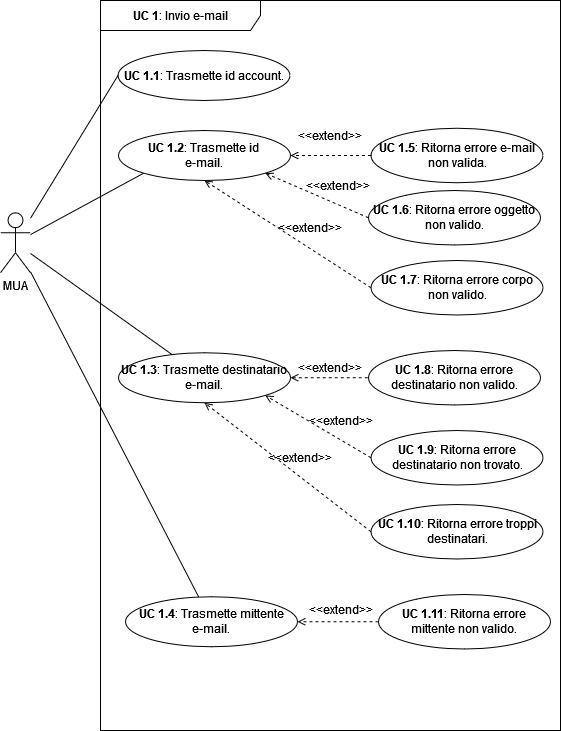
\includegraphics[width=0.85\textwidth]{sections/uc_imgs/UC01.png}
        \centering
        \caption{Diagramma UC 1.}
    \end{figure}
    \begin{itemize}
        \item \textbf{Attore principale}: MUA;
        \item \textbf{Descrizione}: il MUA deve poter inviare una e-mail al destinatario indicato;
        \item \textbf{Precondizioni}: l’account che il MUA gestisce è registrato nel sistema, e ha un connessione aperta con il sistema ed è autenticato;
        \item \textbf{Postcondizioni}: l'e-mail è stata consegnata con successo al destinatario, ed è stata salvata nel sistema;
        \item \textbf{Scenario principale}:
            \begin{enumerate}
                \item il MUA trasmette il destinatario dell'e-mail (\hyperref[sec:UC1.1]{UC 1.1});
                \item il MUA trasmette il mittente dell'e-mail (\hyperref[sec:UC1.2]{UC 1.2});
                \item il MUA trasmette l'oggetto dell'e-mail (\hyperref[sec:UC1.3]{UC 1.3});
                \item il MUA trasmette il corpo dell'e-mail (\hyperref[sec:UC1.4]{UC 1.4});
                \item il sistema salva l'e-mail nel mailbox;
                \item il sistema elabora l'inoltro;
            \end{enumerate}
        \item \textbf{Inclusioni}: nessuna;
        \item \textbf{Generalizzazioni}: nessuna;
        \item \textbf{Estensioni}: 
            \begin{enumerate}[label=\alph*.]
                \item il sistema incontra un errore durante il tentativo d'invio dell'e-mail:
                \begin{enumerate}[label=\arabic*.]
                    \item invia l'e-mail con il codice d'errore al MUA (\hyperref[sec:UC2]{UC 2}).
                \end{enumerate}
            \end{enumerate}
    \end{itemize}

    \begin{figure}[h]
        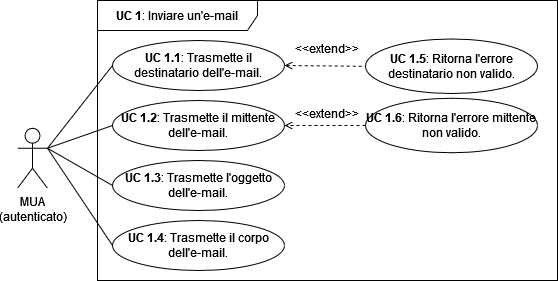
\includegraphics[width=0.75\textwidth]{sections/uc_imgs/UC01.X.png}
        \centering
        \caption{Diagramma sotto-casi UC 1.}
    \end{figure}

    \subsubsection{UC 1.1 - Trasmette il destinatario dell'e-mail} \label{sec:UC1.1}
    \begin{itemize}
        \item \textbf{Attore}: MUA;
        \item \textbf{Descrizione}: il MUA invia al sistema il destinatario dell'e-mail;
        \item \textbf{Precondizioni}: il MUA sta usando la funzionalità d'invio di un'e-mail;
        \item \textbf{Postcondizioni}: il sistema conosce l'indirizzo di posta elettronica del destinatario dell'e-mail;
        \item \textbf{Scenario principale}:
            \begin{enumerate}
                \item il MUA trasmette il destinatario, deve soddisfare il seguente requisito:
                    \begin{itemize}
                        \item l'indirizzo e-mail deve essere sintatticamente valido;
                    \end{itemize}
            \end{enumerate}
        \item \textbf{Inclusioni}: nessuna;
        \item \textbf{Generalizzazioni}: nessuna;
        \item \textbf{Estensioni}:
            \begin{enumerate}[label=\alph*.]
                \item l'indirizzo e-mail non è sintatticamente valido:
                \begin{enumerate}[label=\arabic*.]
                    \item il sistema invia un messaggio di errore al MUA (\hyperref[sec:UC1.6]{UC 1.6}).
                \end{enumerate}
            \end{enumerate}
    \end{itemize}

    \subsubsection{UC 1.2 - Trasmette il mittente dell'e-mail} \label{sec:UC1.2}
    \begin{itemize}
        \item \textbf{Attore}: MUA;
        \item \textbf{Descrizione}: il MUA invia al sistema il mittente dell'e-mail;
        \item \textbf{Precondizioni}: il MUA sta usando la funzionalità d'invio di un'e-mail;
        \item \textbf{Postcondizioni}: il sistema conosce l'indirizzo di posta elettronica del mittente dell'e-mail;
        \item \textbf{Scenario principale}:
            \begin{enumerate}
                \item il MUA trasmette il mittente, deve soddisfare il seguente requisito:
                    \begin{itemize}
                        \item l'indirizzo e-mail deve essere sintatticamente valido;
                    \end{itemize}
            \end{enumerate}
        \item \textbf{Inclusioni}: nessuna;
        \item \textbf{Generalizzazioni}: nessuna;
        \item \textbf{Estensioni}:
            \begin{enumerate}[label=\alph*.]
                \item l'indirizzo e-mail non è sintatticamente valido:
                \begin{enumerate}[label=\arabic*.]
                    \item il sistema invia un messaggio di errore al MUA (\hyperref[sec:UC1.7]{UC 1.7}).
                \end{enumerate}
            \end{enumerate}
    \end{itemize}

    \subsubsection{UC 1.3 - Trasmette l'oggetto dell'e-mail} \label{sec:UC1.3}
    \begin{itemize}
        \item \textbf{Attore}: MUA;
        \item \textbf{Descrizione}: il MUA invia al sistema l'oggetto dell'e-mail;
        \item \textbf{Precondizioni}: il MUA sta usando la funzionalità d'invio di un'e-mail;
        \item \textbf{Postcondizioni}: il sistema conosce l'oggetto dell'e-mail;
        \item \textbf{Scenario principale}:
            \begin{enumerate}
                \item il MUA trasmette l'oggetto dell'e-mail;
            \end{enumerate}
        \item \textbf{Inclusioni}: nessuna;
        \item \textbf{Generalizzazioni}: nessuna;
        \item \textbf{Estensioni}: nessuna.
    \end{itemize}

    \subsubsection{UC 1.4 - Trasmette il corpo dell'e-mail} \label{sec:UC1.4}
    \begin{itemize}
        \item \textbf{Attore}: MUA;
        \item \textbf{Descrizione}: il MUA invia al sistema il corpo dell'e-mail;
        \item \textbf{Precondizioni}: il MUA sta usando la funzionalità d'invio di un'e-mail;
        \item \textbf{Postcondizioni}: il sistema conosce il corpo dell'e-mail;
        \item \textbf{Scenario principale}:
            \begin{enumerate}
                \item il MUA trasmette il corpo dell'e-mail;
            \end{enumerate}
        \item \textbf{Inclusioni}: nessuna;
        \item \textbf{Generalizzazioni}: nessuna;
        \item \textbf{Estensioni}: nessuna.
    \end{itemize}



    \subsubsection{UC 1.5 - Ritorna l'errore destinatario non valido} \label{sec:UC1.5}
    \begin{itemize}
        \item \textbf{Attore}: MUA;
        \item \textbf{Descrizione}: il MUA riceve l'errore che il destinatario non è valido;
        \item \textbf{Precondizioni}: il MUA ha inviato il destinatario;
        \item \textbf{Postcondizioni}: il MUA viene notificato che il destinatario non è valido;
        \item \textbf{Scenario principale}:
            \begin{enumerate}
                \item il sistema controlla la sintassi del destinatario e trova un errore;
                \item il sistema notifica il MUA che il destinatario non è valido;
            \end{enumerate}
        \item \textbf{Inclusioni}: nessuna;
        \item \textbf{Generalizzazioni}: nessuna;
        \item \textbf{Estensioni}: nessuna.
    \end{itemize}

    \subsubsection{UC 1.6 - Ritorna l'errore mittente non valido} \label{sec:UC1.6}
    \begin{itemize}
        \item \textbf{Attore}: MUA;
        \item \textbf{Descrizione}: il MUA riceve l'errore che il mittente non è valido;
        \item \textbf{Precondizioni}: il MUA ha inviato il mittente;
        \item \textbf{Postcondizioni}: il MUA viene notificato che il mittente non è valido;
        \item \textbf{Scenario principale}:
            \begin{enumerate}
                \item il sistema controlla la sintassi del mittente e trova un errore;
                \item il sistema notifica il MUA che il mittente non è valido;
            \end{enumerate}
        \item \textbf{Inclusioni}: nessuna;
        \item \textbf{Generalizzazioni}: nessuna;
        \item \textbf{Estensioni}: nessuna.
    \end{itemize}



        % \subsubsection{UC 1.5 - Trasmettere gli allegati dell'e-mail} \label{sec:UC1.5}
    % \begin{itemize}
    %     \item \textbf{Attore}: MUA;
    %     \item \textbf{Descrizione}: il MUA invia al sistema il mittente dell'e-mail;
    %     \item \textbf{Precondizioni}: il MUA sta usando la funzionalità d'invio di un'e-mail;
    %     \item \textbf{Postcondizioni}: il sistema conosce l'indirizzo di posta elettronica del mittente dell'e-mail;
    %     \item \textbf{Scenario principale}:
    %         \begin{enumerate}
    %             \item il MUA trasmette gli allegati;
    %         \end{enumerate}
    %     \item \textbf{Inclusioni}: nessuna;
    %     \item \textbf{Generalizzazioni}: nessuna;
    %     \item \textbf{Estensioni}: 
    %         \begin{enumerate}[label=\alph*.]
    %             \item l'allegato supera la dimensione massima supporta dal sistema:
    %                 \begin{enumerate}[label=\arabic*.]
    %                     \item il sistema invia un messaggio di errore al MUA (\hyperref[sec:UC1.6]{UC 1.6}).
    %                 \end{enumerate}
    %         \end{enumerate}
    % \end{itemize}

    % \subsubsection{UC 1.8 - Ritorna l'errore massima dimensione allegati} \label{sec:UC1.8}
    % \begin{itemize}
    %     \item \textbf{Attore}: MUA;
    %     \item \textbf{Descrizione}: il MUA viene notificato che gli allegati dell'e-mail hanno superato la massima dimensione supportata;
    %     \item \textbf{Precondizioni}: il MUA sta usando di trasmissione degli allegati;
    %     \item \textbf{Postcondizioni}: il MUA è stato notificato del superamento della massima dimensione per gli allegati;
    %     \item \textbf{Scenario principale}:
    %         \begin{enumerate}
    %             \item il sistema controlla la dimensione degli allegati;
    %             \item il sistema nota che la dimensione è stata superata;
    %             \item il sistema notifica il MUA che la dimensione degli allegati supera la massima dimensione consentita per un e-mail;
    %         \end{enumerate}
    %     \item \textbf{Inclusioni}: nessuna;
    %     \item \textbf{Generalizzazioni}: nessuna;
    %     \item \textbf{Estensioni}: nessuna.
    % \end{itemize}
    
%LTeX: language=it
\subsection{UC 2 - Creare un'e-mail} \label{sec:UC2}
    \begin{figure}[h]
        %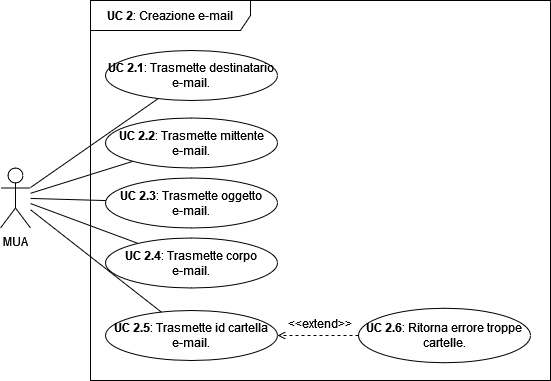
\includegraphics[width=0.85\textwidth]{sections/uc_imgs/UC02.png}
        \centering
        \caption{Diagramma UC 2.}
    \end{figure}
    \begin{itemize}
        \item \textbf{Attore principale}: MUA;
        \item \textbf{Descrizione}: il MUA deve poter inviare una e-mail al destinatario indicato;
        \item \textbf{Precondizioni}: l’account che il MUA gestisce è registrato nel sistema, e ha un connessione aperta con il sistema ed è autenticato;
        \item \textbf{Postcondizioni}: l'e-mail è stata consegnata con successo al destinatario, ed è stata salvata nel sistema;
        \item \textbf{Scenario principale}:
            \begin{enumerate}
                \item il MUA trasmette il destinatario dell'e-mail (\hyperref[sec:UC2.1]{UC 2.1});
                \item il MUA trasmette il mittente dell'e-mail (\hyperref[sec:UC2.2]{UC 2.2});
                \item il MUA trasmette l'oggetto dell'e-mail (\hyperref[sec:UC2.3]{UC 2.3});
                \item il MUA trasmette il corpo dell'e-mail (\hyperref[sec:UC2.4]{UC 2.4});
                \item il sistema salva l'e-mail nel mailbox;
                \item il sistema elabora l'inoltro;
            \end{enumerate}
        \item \textbf{Inclusioni}: nessuna;
        \item \textbf{Generalizzazioni}: nessuna;
        \item \textbf{Estensioni}: 
            \begin{enumerate}[label=\alph*.]
                \item il sistema incontra un errore durante il tentativo d'invio dell'e-mail:
                \begin{enumerate}[label=\arabic*.]
                    \item invia l'e-mail con il codice d'errore al MUA (\hyperref[sec:UC2]{UC 2}).
                \end{enumerate}
            \end{enumerate}
    \end{itemize}

    \begin{figure}[h]
        %\includegraphics[width=0.75\textwidth]{sections/uc_imgs/UC02.X.png}
        \centering
        \caption{Diagramma sotto-casi UC 2.}
    \end{figure}

    \subsubsection{UC 2.1 - Trasmette il destinatario dell'e-mail} \label{sec:UC2.1}
    \begin{itemize}
        \item \textbf{Attore}: MUA;
        \item \textbf{Descrizione}: il MUA invia al sistema il destinatario dell'e-mail;
        \item \textbf{Precondizioni}: il MUA sta usando la funzionalità d'invio di un'e-mail;
        \item \textbf{Postcondizioni}: il sistema conosce l'indirizzo di posta elettronica del destinatario dell'e-mail;
        \item \textbf{Scenario principale}:
            \begin{enumerate}
                \item il MUA trasmette il destinatario, deve soddisfare il seguente requisito:
                    \begin{itemize}
                        \item l'indirizzo e-mail deve essere sintatticamente valido;
                    \end{itemize}
            \end{enumerate}
        \item \textbf{Inclusioni}: nessuna;
        \item \textbf{Generalizzazioni}: nessuna;
        \item \textbf{Estensioni}:
            \begin{enumerate}[label=\alph*.]
                \item l'indirizzo e-mail non è sintatticamente valido:
                \begin{enumerate}[label=\arabic*.]
                    \item il sistema invia un messaggio di errore al MUA (\hyperref[sec:UC2.6]{UC 2.6}).
                \end{enumerate}
            \end{enumerate}
    \end{itemize}

    \subsubsection{UC 2.2 - Trasmette il mittente dell'e-mail} \label{sec:UC2.2}
    \begin{itemize}
        \item \textbf{Attore}: MUA;
        \item \textbf{Descrizione}: il MUA invia al sistema il mittente dell'e-mail;
        \item \textbf{Precondizioni}: il MUA sta usando la funzionalità d'invio di un'e-mail;
        \item \textbf{Postcondizioni}: il sistema conosce l'indirizzo di posta elettronica del mittente dell'e-mail;
        \item \textbf{Scenario principale}:
            \begin{enumerate}
                \item il MUA trasmette il mittente, deve soddisfare il seguente requisito:
                    \begin{itemize}
                        \item l'indirizzo e-mail deve essere sintatticamente valido;
                    \end{itemize}
            \end{enumerate}
        \item \textbf{Inclusioni}: nessuna;
        \item \textbf{Generalizzazioni}: nessuna;
        \item \textbf{Estensioni}:
            \begin{enumerate}[label=\alph*.]
                \item l'indirizzo e-mail non è sintatticamente valido:
                \begin{enumerate}[label=\arabic*.]
                    \item il sistema invia un messaggio di errore al MUA (\hyperref[sec:UC2.7]{UC 2.7}).
                \end{enumerate}
            \end{enumerate}
    \end{itemize}

    \subsubsection{UC 2.3 - Trasmette l'oggetto dell'e-mail} \label{sec:UC2.3}
    \begin{itemize}
        \item \textbf{Attore}: MUA;
        \item \textbf{Descrizione}: il MUA invia al sistema l'oggetto dell'e-mail;
        \item \textbf{Precondizioni}: il MUA sta usando la funzionalità d'invio di un'e-mail;
        \item \textbf{Postcondizioni}: il sistema conosce l'oggetto dell'e-mail;
        \item \textbf{Scenario principale}:
            \begin{enumerate}
                \item il MUA trasmette l'oggetto dell'e-mail;
            \end{enumerate}
        \item \textbf{Inclusioni}: nessuna;
        \item \textbf{Generalizzazioni}: nessuna;
        \item \textbf{Estensioni}: nessuna.
    \end{itemize}

    \subsubsection{UC 2.4 - Trasmette il corpo dell'e-mail} \label{sec:UC2.4}
    \begin{itemize}
        \item \textbf{Attore}: MUA;
        \item \textbf{Descrizione}: il MUA invia al sistema il corpo dell'e-mail;
        \item \textbf{Precondizioni}: il MUA sta usando la funzionalità d'invio di un'e-mail;
        \item \textbf{Postcondizioni}: il sistema conosce il corpo dell'e-mail;
        \item \textbf{Scenario principale}:
            \begin{enumerate}
                \item il MUA trasmette il corpo dell'e-mail;
            \end{enumerate}
        \item \textbf{Inclusioni}: nessuna;
        \item \textbf{Generalizzazioni}: nessuna;
        \item \textbf{Estensioni}: nessuna.
    \end{itemize}



    \subsubsection{UC 2.5 - Ritorna l'errore destinatario non valido} \label{sec:UC2.5}
    \begin{itemize}
        \item \textbf{Attore}: MUA;
        \item \textbf{Descrizione}: il MUA riceve l'errore che il destinatario non è valido;
        \item \textbf{Precondizioni}: il MUA ha inviato il destinatario;
        \item \textbf{Postcondizioni}: il MUA viene notificato che il destinatario non è valido;
        \item \textbf{Scenario principale}:
            \begin{enumerate}
                \item il sistema controlla la sintassi del destinatario e trova un errore;
                \item il sistema notifica il MUA che il destinatario non è valido;
            \end{enumerate}
        \item \textbf{Inclusioni}: nessuna;
        \item \textbf{Generalizzazioni}: nessuna;
        \item \textbf{Estensioni}: nessuna.
    \end{itemize}

    \subsubsection{UC 2.6 - Ritorna l'errore mittente non valido} \label{sec:UC2.6}
    \begin{itemize}
        \item \textbf{Attore}: MUA;
        \item \textbf{Descrizione}: il MUA riceve l'errore che il mittente non è valido;
        \item \textbf{Precondizioni}: il MUA ha inviato il mittente;
        \item \textbf{Postcondizioni}: il MUA viene notificato che il mittente non è valido;
        \item \textbf{Scenario principale}:
            \begin{enumerate}
                \item il sistema controlla la sintassi del mittente e trova un errore;
                \item il sistema notifica il MUA che il mittente non è valido;
            \end{enumerate}
        \item \textbf{Inclusioni}: nessuna;
        \item \textbf{Generalizzazioni}: nessuna;
        \item \textbf{Estensioni}: nessuna.
    \end{itemize}

    %LTeX: language=it
\subsection{UC 3 - Creazione cartella} \label{sec:UC3}
    \begin{itemize}
        \item \textbf{Attore principale}: MUA;
        \item \textbf{Descrizione}: il MUA deve poter creare una cartella nel sistema;
        \item \textbf{Precondizioni}: l’account che il MUA gestisce è registrato nel sistema, e ha una connessione aperta con il sistema ed è autenticato;
        \item \textbf{Postcondizioni}: il MUA crea la cartella che viene salvata nel sistema;
        \item \textbf{Scenario principale}:
            \begin{enumerate}
                \item il MUA trasmette il nome della cartella (\hyperref[sec:UC3.1]{UC 3.1});
                \item il MUA trasmette l'id della cartella genitore (\hyperref[sec:UC3.2]{UC 3.2});
                \item il sistema salva la nuova cartella.
            \end{enumerate}
        \item \textbf{Inclusioni}: nessuna;
        \item \textbf{Generalizzazioni}: nessuna;
        \item \textbf{Estensioni}: nessuna.
    \end{itemize}

\begin{figure}[H]
    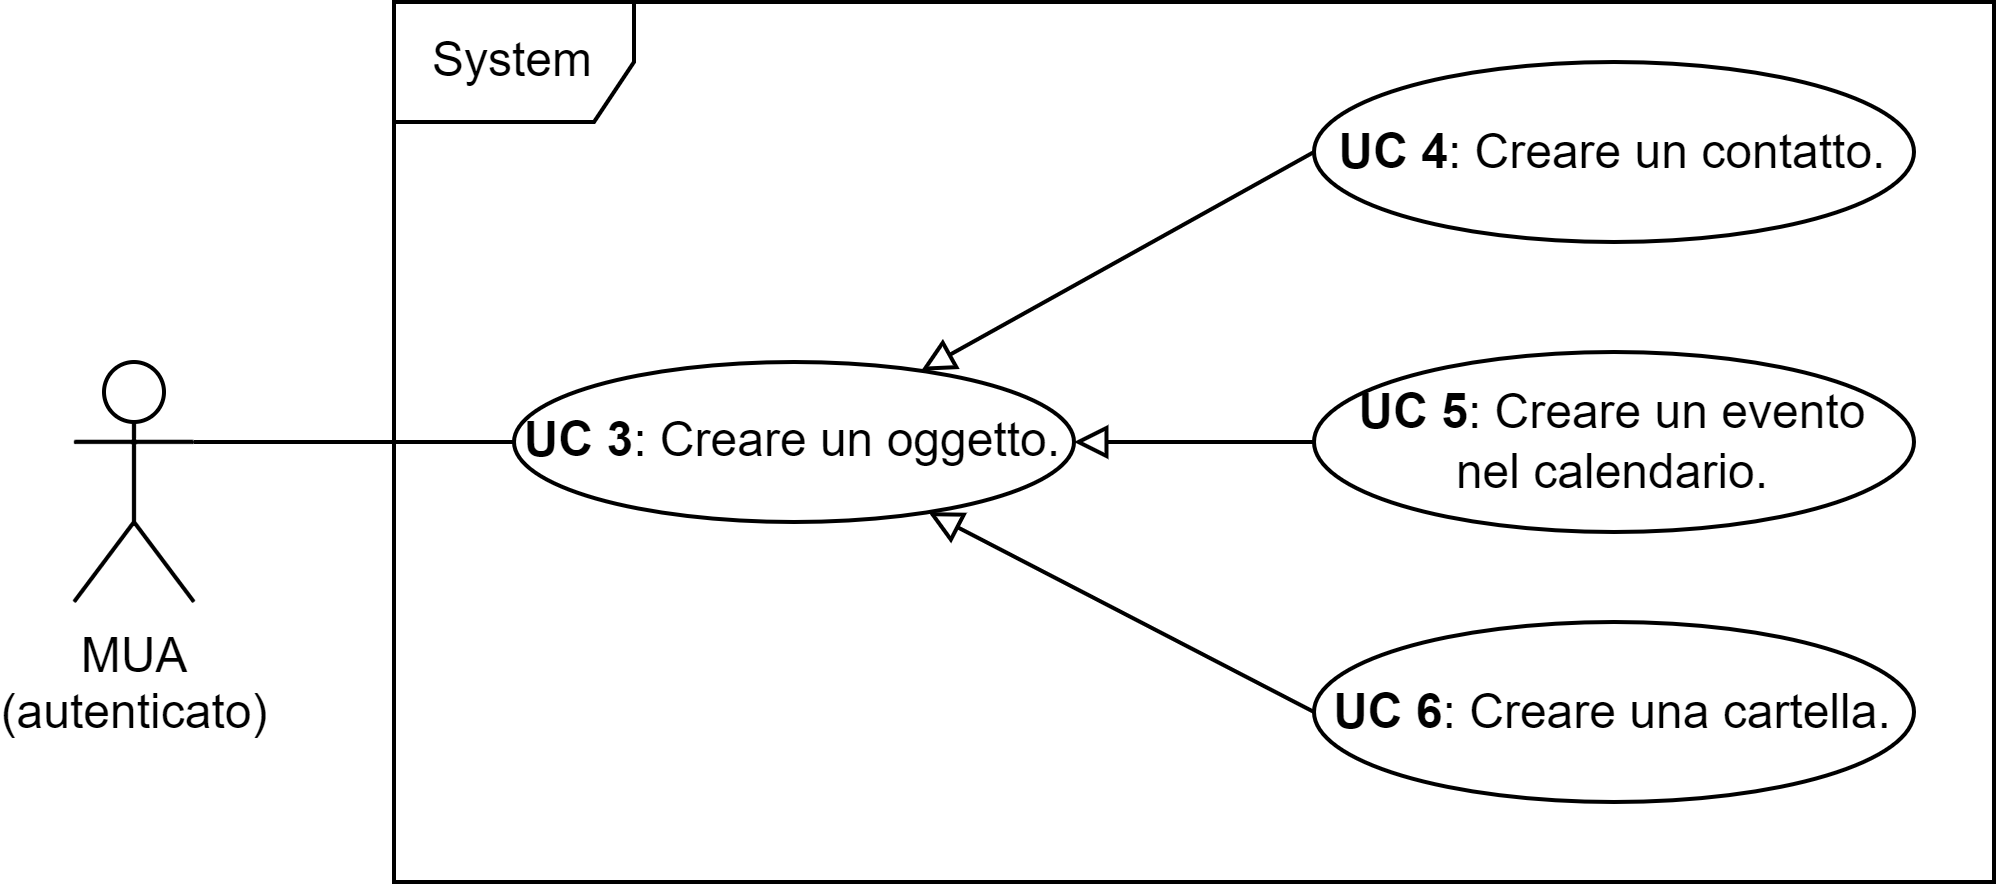
\includegraphics[width=0.85\textwidth]{sections/uc_imgs/UC03.png}
    \centering
    \caption{Diagramma sotto-casi UC 3}
\end{figure}

\subsubsection{UC 3.1 - Trasmette nome cartella} \label{sec:UC3.1}
    \begin{itemize}
        \item \textbf{Attore principale}: MUA;
        \item \textbf{Descrizione}: il MUA trasmette il nome per creare la cartella al sistema;
        \item \textbf{Precondizioni}: il MUA sta usando la funzionalità di creazione di una cartella;
        \item \textbf{Postcondizioni}: il sistema conosce il nome della cartella;
        \item \textbf{Scenario principale}:
            \begin{enumerate}
                \item il MUA invia il nome per creare la cartella al sistema;
                \item il sistema controlla che le informazioni ricevute rispettino il seguente requisito minimo:
                \begin{itemize}
                    \item il nome ricevuto non è una stringa vuota.
                \end{itemize}
            \end{enumerate}
        \item \textbf{Inclusioni}: nessuna;
        \item \textbf{Generalizzazioni}: nessuna;
        \item \textbf{Estensioni}:
            \begin{enumerate}[label=\alph*.]
                \item il sistema non riesce a creare la cartella perché il nome fornito non è valido:
                \begin{enumerate}[label=\arabic*.]
                    \item il sistema ritorna un errore al MUA di nome non valido (\hyperref[sec:UC3.3]{UC 3.3}).
                \end{enumerate}
            \end{enumerate}
    \end{itemize}

    \subsubsection{UC 3.2 - Trasmette id cartella genitore} \label{sec:UC3.2}
    \begin{itemize}
        \item \textbf{Attore principale}: MUA;
        \item \textbf{Descrizione}: il MUA trasmette l'id della cartella genitore al sistema;
        \item \textbf{Precondizioni}: il MUA sta usando la funzionalità di creazione di una cartella;
        \item \textbf{Postcondizioni}: il sistema conosce l'id della cartella genitore;
        \item \textbf{Scenario principale}:
            \begin{enumerate}
                \item il MUA invia le informazioni necessarie per creare la cartella;
                \item il sistema elabora le informazioni ricevute, controlla che:
                \begin{itemize}
                    \item la cartella genitore esista.
                \end{itemize}
            \end{enumerate}
        \item \textbf{Inclusioni}: nessuna;
        \item \textbf{Generalizzazioni}: nessuna;
        \item \textbf{Estensioni}:
            \begin{enumerate}[label=\alph*.]
                \item il sistema non riesce a salvare la cartella perché non trova la cartella genitore:
                \begin{enumerate}[label=\arabic*.]
                    \item il sistema ritorna un errore al MUA di cartella genitore non trovata (\hyperref[sec:UC3.4]{UC 3.4});
                    \end{enumerate}
                \item il sistema non riesce a salvare la cartella perché è un duplicato:
                \begin{enumerate}[label=\arabic*.]
                    \item il sistema ritorna un errore al MUA di cartella duplicata (\hyperref[sec:UC3.5]{UC 3.5}).
                \end{enumerate}
                
            \end{enumerate}
    \end{itemize}



    \subsubsection{UC 3.3 - Ritorna errore nome non valido} \label{sec:UC3.3}
    \begin{itemize}
        \item \textbf{Attore principale}: MUA;
        \item \textbf{Descrizione}: il MUA riceve l'errore che il nome della cartella non è valido;
        \item \textbf{Precondizioni}:  il MUA ha trasmesso il nome per creare la cartella al sistema;
        \item \textbf{Postcondizioni}: il sistema non crea la nuova cartella e il MUA viene notificato dell'errore;
        \item \textbf{Scenario principale}:
            \begin{enumerate}
                \item il sistema controlla la sintassi del nome e trova un errore;
                \item il sistema non crea la cartella e notifica il MUA dell'errore.
            \end{enumerate}
        \item \textbf{Inclusioni}: nessuna;
        \item \textbf{Generalizzazioni}: nessuna;
        \item \textbf{Estensioni}: nessuna.
    \end{itemize}

    \subsubsection{UC 3.4 - Ritorna errore cartella genitore non trovata} \label{sec:UC3.4}
    \begin{itemize}
        \item \textbf{Attore principale}: MUA;
        \item \textbf{Descrizione}: il MUA riceve l'errore che la cartella genitore non è stata trovata;
        \item \textbf{Precondizioni}: il MUA ha trasmesso l'id della cartella genitore al sistema;
        \item \textbf{Postcondizioni}: il sistema non crea la nuova cartella e il MUA viene notificato dell'errore;
        \item \textbf{Scenario principale}:
            \begin{enumerate}
                \item il sistema non trova l'di fornito;
                \item il sistema non crea la cartella e notifica il MUA dell'errore.
            \end{enumerate}
        \item \textbf{Inclusioni}: nessuna;
        \item \textbf{Generalizzazioni}: nessuna;
        \item \textbf{Estensioni}: nessuna.
    \end{itemize}

\subsubsection{UC 3.5 - Ritorna errore cartella duplicata} \label{sec:UC3.5}
    \begin{itemize}
        \item \textbf{Attore principale}: MUA;
        \item \textbf{Descrizione}: il MUA riceve l'errore che la cartella è duplicata;
        \item \textbf{Precondizioni}: il MUA ha trasmesso i dettagli per creare la cartella al sistema;
        \item \textbf{Postcondizioni}: il sistema non crea la nuova cartella e il MUA viene notificato dell'errore;
        \item \textbf{Scenario principale}:
            \begin{enumerate}
                \item il sistema nota che la cartella esiste già e annulla l'operazione per la creazione della cartella;
                \item il sistema non crea la cartella e notifica il MUA dell'errore.
            \end{enumerate}
        \item \textbf{Inclusioni}: nessuna;
        \item \textbf{Generalizzazioni}: nessuna;
        \item \textbf{Estensioni}: nessuna.
    \end{itemize}


    %LTeX: language=it
\subsection{UC 4 - Creazione contatto} \label{sec:UC4}
    \begin{itemize}
        \item \textbf{Attore principale}: MUA;
        \item \textbf{Descrizione}: il MUA deve poter creare un contatto nel sistema;
        \item \textbf{Precondizioni}: l’account che il MUA gestisce è registrato nel sistema, ha una connessione aperta con il sistema ed è autenticato;
        \item \textbf{Postcondizioni}: il MUA crea il contatto che viene salvato nel sistema;
        \item \textbf{Scenario principale}:
            \begin{enumerate}
                \item il MUA trasmette il nome del contatto (\hyperref[sec:UC4.1]{UC 4.1});
                \item il MUA trasmette l'indirizzo e-mail del contatto (\hyperref[sec:UC4.2]{UC 4.2});
                \item il sistema salva il contatto;
            \end{enumerate}
        \item \textbf{Inclusioni}: nessuna;
        \item \textbf{Generalizzazioni}: nessuna;
        \item \textbf{Estensioni}: nessuna.
    \end{itemize}

\begin{figure}[H]
    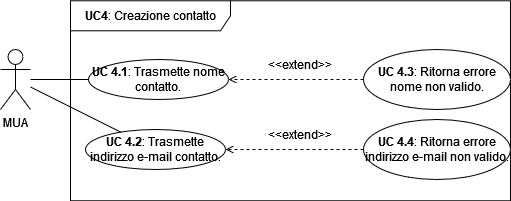
\includegraphics[width=0.85\textwidth]{sections/uc_imgs/UC04.png}
    \centering
    \caption{Diagramma sotto-casi UC 4}
\end{figure}

\subsubsection{UC 4.1 - Trasmette nome contatto} \label{sec:UC4.1}
    \begin{itemize}
        \item \textbf{Attore principale}: MUA;
        \item \textbf{Descrizione}: il MUA trasmette il nome per creare il contatto al sistema;
        \item \textbf{Precondizioni}: il MUA sta usando la funzionalità di creazione di un contatto;
        \item \textbf{Postcondizioni}: il sistema conosce il nome del contatto;
        \item \textbf{Scenario principale}:
            \begin{enumerate}
                \item il MUA invia il nome per creare il contatto al sistema;
                \item il sistema controlla che le informazioni ricevute rispettino il seguente requisito minimo:
                    \begin{itemize}
                        \item il nome del contatto non è una stringa vuota;
                    \end{itemize}
            \end{enumerate}
        \item \textbf{Inclusioni}: nessuna;
        \item \textbf{Generalizzazioni}: nessuna;
        \item \textbf{Estensioni}:
            \begin{enumerate}[label=\alph*.]
                \item il sistema non riesce a creare il contatto perché il nome fornito non è valido:
                \begin{enumerate}[label=\arabic*.]
                    \item il sistema ritorna un errore al MUA di nome non valido (\hyperref[sec:UC4.3]{UC 4.3}).
                \end{enumerate}
            \end{enumerate}
    \end{itemize}


    \subsubsection{UC 4.2 - Trasmette indirizzo e-mail contatto} \label{sec:UC4.2}
    \begin{itemize}
        \item \textbf{Attore principale}: MUA;
        \item \textbf{Descrizione}: il MUA trasmette l'indirizzo e-mail per creare il contatto al sistema;
        \item \textbf{Precondizioni}: il MUA sta usando la funzionalità di creazione di un contatto;
        \item \textbf{Postcondizioni}: il sistema conosce l'indirizzo e-mail del contatto;
        \item \textbf{Scenario principale}:
            \begin{enumerate}
                \item il MUA invia l'indirizzo e-mail per creare il contatto al sistema;
                \item il sistema controlla che le informazioni ricevute rispettino il seguente requisito minimo:
                    \begin{itemize}
                        \item l'indirizzo e-mail del contatto non è una stringa vuota;
                    \end{itemize}
            \end{enumerate}
        \item \textbf{Inclusioni}: nessuna;
        \item \textbf{Generalizzazioni}: nessuna;
        \item \textbf{Estensioni}:
            \begin{enumerate}[label=\alph*.]
                \item il sistema non riesce a creare il contatto perché l'indirizzo e-mail fornito non è valido:
                \begin{enumerate}[label=\arabic*.]
                    \item il sistema ritorna un errore al MUA di indirizzo e-mail non valido (\hyperref[sec:UC4.4]{UC 4.4}).
                \end{enumerate}
            \end{enumerate}
    \end{itemize}




\subsubsection{UC 4.3 - Ritorna errore nome non valido} \label{sec:UC4.3}
    \begin{itemize}
        \item \textbf{Attore principale}: MUA;
        \item \textbf{Descrizione}: il sistema non riesce a salvare il contatto perché il nome del contatto non rispetta i requisiti;
        \item \textbf{Precondizioni}: il MUA ha inviato il nome del contatto;
        \item \textbf{Postcondizioni}: il sistema non salva il nuovo contatto, il MUA è stato notificato dell'errore;
        \item \textbf{Scenario principale}:
            \begin{enumerate}
                \item il sistema controlla la sintassi del nome del contatto e trova un errore;
                \item il sistema non salva il contatto e notifica il MUA dell'errore;
            \end{enumerate}
        \item \textbf{Inclusioni}: nessuna;
        \item \textbf{Generalizzazioni}: nessuna;
        \item \textbf{Estensioni}: nessuna.
    \end{itemize}

\subsubsection{UC 4.4 - Ritorna errore indirizzo e-mail non valido} \label{sec:UC4.4}
    \begin{itemize}
        \item \textbf{Attore principale}: MUA;
        \item \textbf{Descrizione}: il sistema non riesce a salvare il contatto perché l'indirizzo e-mail del contatto non rispetta i requisiti;
        \item \textbf{Precondizioni}: il MUA ha inviato l'indirizzo e-mail del contatto;
        \item \textbf{Postcondizioni}: il sistema non salva il nuovo contatto, il MUA è stato notificato dell'errore;
        \item \textbf{Scenario principale}:
            \begin{enumerate}
                \item il sistema controlla la sintassi dell'indirizzo e-mail del contatto e trova un errore;
                \item il sistema non salva il contatto e notifica il MUA dell'errore;
            \end{enumerate}
        \item \textbf{Inclusioni}: nessuna;
        \item \textbf{Generalizzazioni}: nessuna;
        \item \textbf{Estensioni}: nessuna.
    \end{itemize}
    %LTeX: language=it
\subsection{UC 5 - Creazione evento} \label{sec:UC5}
    \begin{itemize}
        \item \textbf{Attore principale}: MUA;
        \item \textbf{Descrizione}: il MUA deve poter creare un evento nel sistema;
        \item \textbf{Precondizioni}: l’account che il MUA gestisce è registrato nel sistema, ha una connessione aperta con il sistema ed è autenticato;
        \item \textbf{Postcondizioni}: il MUA crea l'evento che viene salvato nel sistema;
        \item \textbf{Scenario principale}:
            \begin{enumerate}
                \item il MUA trasmette il titolo dell'evento (\hyperref[sec:UC5.1]{UC 5.1});
                \item il MUA trasmette la data di inizio dell'evento (\hyperref[sec:UC5.2]{UC 5.2});
                \item il MUA trasmette la data di fine dell'evento (\hyperref[sec:UC5.3]{UC 5.3});
                \item il MUA trasmette la durata dell'evento (\hyperref[sec:UC5.4]{UC 5.4});
                \item il sistema salva l'evento;
            \end{enumerate}
        \item \textbf{Inclusioni}: nessuna;
        \item \textbf{Generalizzazioni}: nessuna;
        \item \textbf{Estensioni}: nessuna.
    \end{itemize}

\begin{figure}[H]
    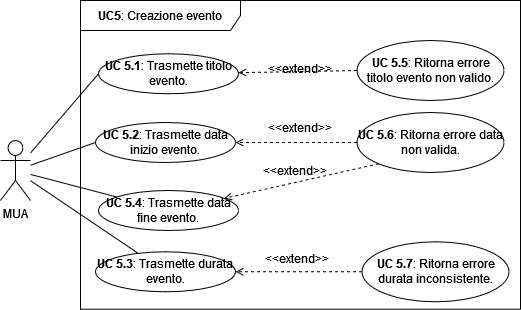
\includegraphics[width=0.85\textwidth]{sections/uc_imgs/UC05.png}
    \centering
    \caption{Diagramma sotto-casi UC 5}
\end{figure}

\subsubsection{UC 5.1 - Trasmette titolo evento} \label{sec:UC5.1}
    \begin{itemize}
        \item \textbf{Attore principale}: MUA;
        \item \textbf{Descrizione}: il MUA trasmette il titolo per creare l'evento al sistema;
        \item \textbf{Precondizioni}: il MUA sta usando la funzionalità di creazione di un evento;
        \item \textbf{Postcondizioni}: il sistema conosce il titolo dell'evento;
        \item \textbf{Scenario principale}:
            \begin{enumerate}
                \item il MUA invia il titolo per creare l'evento al sistema;
                \item il sistema controlla che le informazioni ricevute rispettino il seguente requisito minimo:
                    \begin{itemize}
                        \item il titolo dell'evento non è una stringa vuota;
                    \end{itemize}
            \end{enumerate}
        \item \textbf{Inclusioni}: nessuna;
        \item \textbf{Generalizzazioni}: nessuna;
        \item \textbf{Estensioni}:
            \begin{enumerate}[label=\alph*.]
                \item il sistema non riesce a creare l'evento perché il titolo fornito non è valido:
                \begin{enumerate}[label=\arabic*.]
                    \item il sistema ritorna un errore al MUA di titolo evento non valido (\hyperref[sec:UC5.5]{UC 5.5}).
                \end{enumerate}
            \end{enumerate}
    \end{itemize}



    \subsubsection{UC 5.2 - Trasmette data inizio evento} \label{sec:UC5.2}
    \begin{itemize}
        \item \textbf{Attore principale}: MUA;
        \item \textbf{Descrizione}: il MUA trasmette la data di inizio dell'evento per creare l'evento al sistema;
        \item \textbf{Precondizioni}: il MUA sta usando la funzionalità di creazione di un evento;
        \item \textbf{Postcondizioni}: il sistema conosce la data di inizio dell'evento;
        \item \textbf{Scenario principale}:
            \begin{enumerate}
                \item il MUA invia la data di inizio dell'evento per creare l'evento al sistema;
                \item il sistema controlla che le informazioni ricevute rispettino il seguente requisito minimo:
                    \begin{itemize}
                        \item la data di inizio dell'evento è in un formato corretto;
                    \end{itemize}
            \end{enumerate}
        \item \textbf{Inclusioni}: nessuna;
        \item \textbf{Generalizzazioni}: nessuna;
        \item \textbf{Estensioni}:
            \begin{enumerate}[label=\alph*.]
                \item il sistema non riesce a creare l'evento perché la data di inizio dell'evento fornita non è in un formato corretto:
                \begin{enumerate}[label=\arabic*.]
                    \item il sistema ritorna un errore al MUA di data evento non valida (\hyperref[sec:UC5.6]{UC 5.6}).
                \end{enumerate}
            \end{enumerate}
    \end{itemize}


    \subsubsection{UC 5.3 - Trasmette data fine evento} \label{sec:UC5.3}
    \begin{itemize}
        \item \textbf{Attore principale}: MUA;
        \item \textbf{Descrizione}: il MUA trasmette la data di fine dell'evento per creare l'evento al sistema;
        \item \textbf{Precondizioni}: il MUA sta usando la funzionalità di creazione di un evento;
        \item \textbf{Postcondizioni}: il sistema conosce la data di fine dell'evento;
        \item \textbf{Scenario principale}:
            \begin{enumerate}
                \item il MUA invia la data di fine dell'evento per creare l'evento al sistema;
                \item il sistema controlla che le informazioni ricevute rispettino il seguente requisito minimo:
                    \begin{itemize}
                        \item la data di fine dell'evento è in un formato corretto;
                    \end{itemize}
            \end{enumerate}
        \item \textbf{Inclusioni}: nessuna;
        \item \textbf{Generalizzazioni}: nessuna;
        \item \textbf{Estensioni}:
            \begin{enumerate}[label=\alph*.]
                \item il sistema non riesce a creare l'evento perché la data di fine dell'evento fornita non è in un formato corretto:
                \begin{enumerate}[label=\arabic*.]
                    \item il sistema ritorna un errore al MUA di data evento non valida (\hyperref[sec:UC5.6]{UC 5.6}).
                \end{enumerate}
            \end{enumerate}
    \end{itemize}

    \subsubsection{UC 5.4 - Trasmette durata evento} \label{sec:UC5.4}
    \begin{itemize}
        \item \textbf{Attore principale}: MUA;
        \item \textbf{Descrizione}: il MUA trasmette la durata per creare l'evento al sistema;
        \item \textbf{Precondizioni}: il MUA sta usando la funzionalità di creazione di un evento;
        \item \textbf{Postcondizioni}: il sistema conosce la durata dell'evento;
        \item \textbf{Scenario principale}:
            \begin{enumerate}
                \item il MUA invia la durata per creare l'evento al sistema;
                \item il sistema controlla che le informazioni ricevute rispettino il seguente requisito minimo:
                    \begin{itemize}
                        \item la durata dell'evento deve essere consistente con la data di inizio e la data di fine;
                    \end{itemize}
            \end{enumerate}
        \item \textbf{Inclusioni}: nessuna;
        \item \textbf{Generalizzazioni}: nessuna;
        \item \textbf{Estensioni}:
            \begin{enumerate}[label=\alph*.]
                \item il sistema non riesce a creare l'evento perché la durata fornita non è valida:
                \begin{enumerate}[label=\arabic*.]
                    \item il sistema ritorna un errore al MUA di durata inconsistente (\hyperref[sec:UC5.7]{UC 5.7}).
                \end{enumerate}
            \end{enumerate}
    \end{itemize}


    \subsubsection{UC 5.5 - Ritorna errore titolo evento non valido} \label{sec:UC5.5}
    \begin{itemize}
        \item \textbf{Attore principale}: MUA;
        \item \textbf{Descrizione}: il sistema non riesce a salvare l'evento perché il titolo dell'evento non rispetta i requisiti;
        \item \textbf{Precondizioni}: il MUA ha inviato il titolo dell'evento;
        \item \textbf{Postcondizioni}: il sistema non salva il nuovo evento, il MUA è stato notificato dell'errore;
        \item \textbf{Scenario principale}:
            \begin{enumerate}
                \item il sistema controlla la sintassi del titolo dell'evento e trova un errore;
                \item il sistema non salva l'evento e notifica il MUA dell'errore;
            \end{enumerate}
        \item \textbf{Inclusioni}: nessuna;
        \item \textbf{Generalizzazioni}: nessuna;
        \item \textbf{Estensioni}: nessuna.
    \end{itemize}


    \subsubsection{UC 5.6 - Ritorna errore data non valida} \label{sec:UC5.6}
    \begin{itemize}
        \item \textbf{Attore principale}: MUA;
        \item \textbf{Descrizione}: il sistema non riesce a salvare l'evento perché la data non rispetta i requisiti;
        \item \textbf{Precondizioni}: il MUA ha inviato il titolo dell'evento;
        \item \textbf{Postcondizioni}: il sistema non salva il nuovo evento, il MUA è stato notificato dell'errore;
        \item \textbf{Scenario principale}:
            \begin{enumerate}
                \item il sistema controlla il formato della data dell'evento e trova un errore;
                \item il sistema non salva l'evento e notifica il MUA dell'errore;
            \end{enumerate}
        \item \textbf{Inclusioni}: nessuna;
        \item \textbf{Generalizzazioni}: nessuna;
        \item \textbf{Estensioni}: nessuna.
    \end{itemize}

    \subsubsection{UC 5.7 - Ritorna errore durata inconsistente} \label{sec:UC5.7}
    \begin{itemize}
        \item \textbf{Attore principale}: MUA;
        \item \textbf{Descrizione}: il sistema non riesce a salvare l'evento perché la durata non rispetta i requisiti;
        \item \textbf{Precondizioni}: il MUA ha inviato la durata dell'evento;
        \item \textbf{Postcondizioni}: il sistema non salva il nuovo evento, il MUA è stato notificato dell'errore;
        \item \textbf{Scenario principale}:
            \begin{enumerate}
                \item il sistema controlla la consistenza della durata e trova un errore;
                \item il sistema non salva l'evento e notifica il MUA dell'errore;
            \end{enumerate}
        \item \textbf{Inclusioni}: nessuna;
        \item \textbf{Generalizzazioni}: nessuna;
        \item \textbf{Estensioni}: nessuna.
    \end{itemize}
    %LTeX: language=it
<<<<<<< HEAD
\subsection{UC 6 - Creazione di una cartella} \label{sec:UC6}
    \begin{itemize}
        \item \textbf{Attore principale}: MUA;
        \item \textbf{Descrizione}: il MUA crea una cartella nel sistema;
        \item \textbf{Precondizioni}: il MUA sta usando la funzionalità di creazione di un oggetto;
        \item \textbf{Postcondizioni}: il sistema salva la nuova cartella creata;
        \item \textbf{Scenario principale}:
            \begin{enumerate}
                \item il MUA invia le informazioni per creare la cartella (\hyperref[sec:UC6.1]{UC 6.1});
                \item il sistema salva la nuova cartella;
            \end{enumerate}
        \item \textbf{Inclusioni}: nessuna;
        \item \textbf{Generalizzazioni}: nessuna;
        \item \textbf{Estensioni}: nessuna.
    \end{itemize}

\begin{figure}[h]
    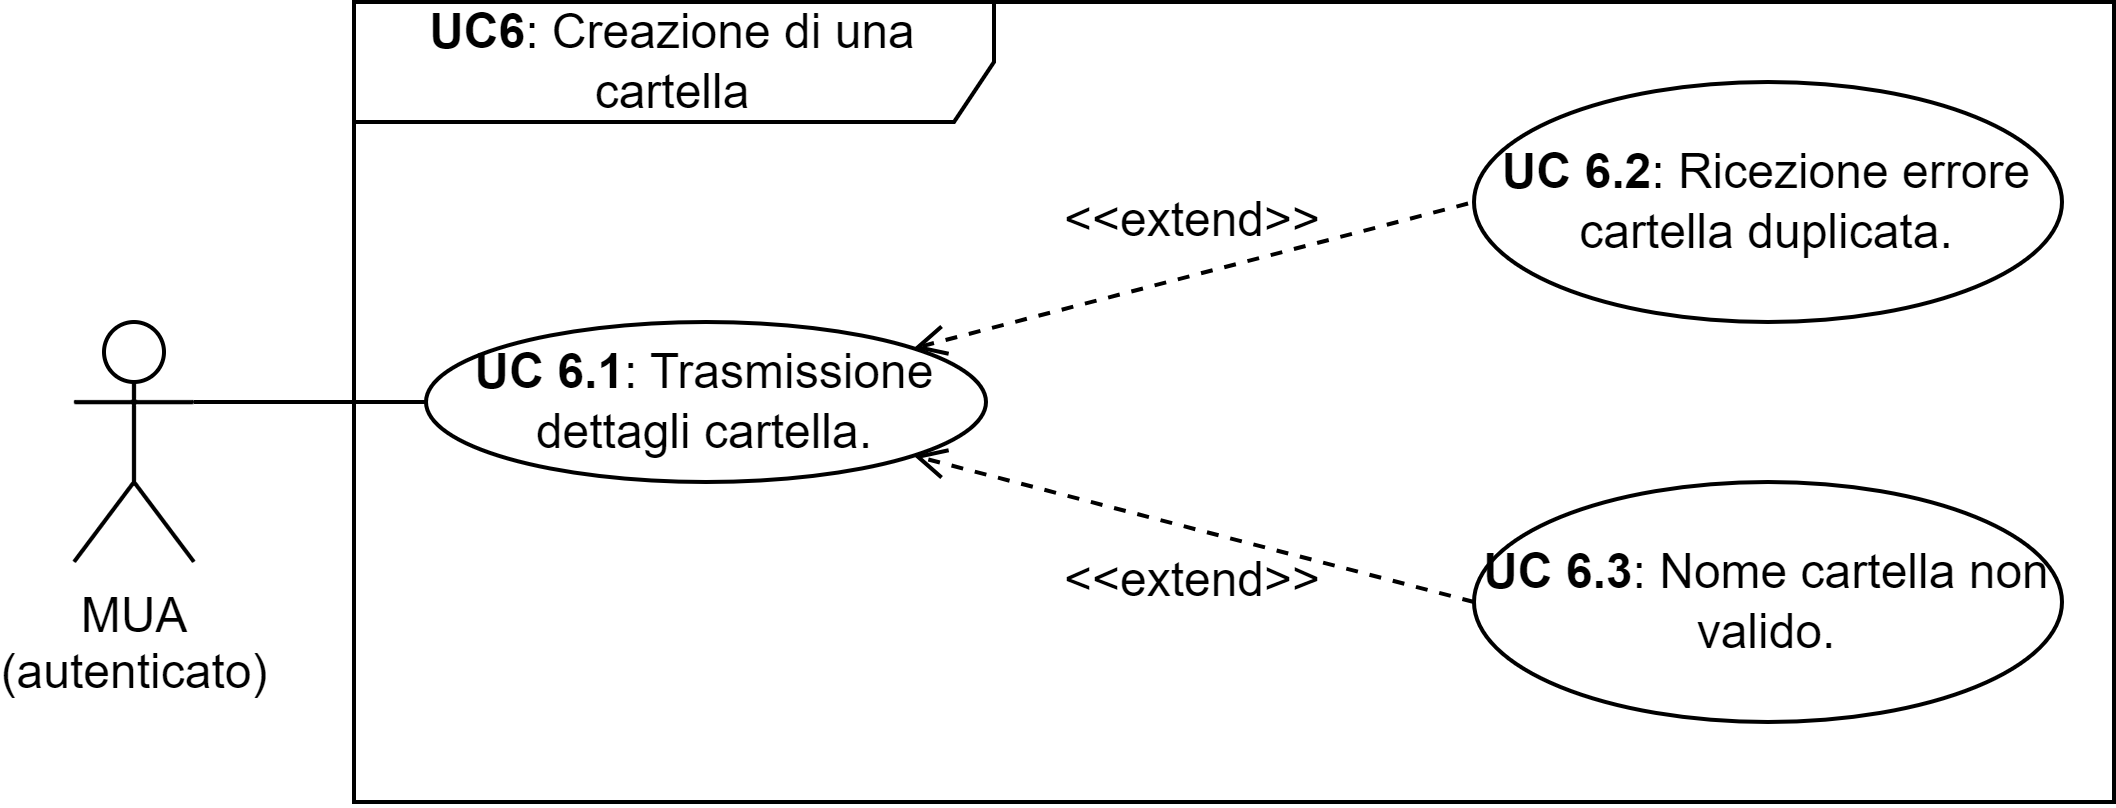
\includegraphics[width=0.85\textwidth]{sections/uc_imgs/UC06.X.png}
    \centering
    \caption{Diagramma sotto-casi UC 6.}
\end{figure}

\subsubsection{UC 6.1 - Trasmette dettagli della cartella} \label{sec:UC6.1}
    \begin{itemize}
        \item \textbf{Attore principale}: MUA;
        \item \textbf{Descrizione}: il MUA trasmette i dettagli per creare la cartella al sistema;
        \item \textbf{Precondizioni}: il MUA sta usando la funzionalità di creazione di una cartella;
        \item \textbf{Postcondizioni}: il sistema salva la nuova cartella creata;
        \item \textbf{Scenario principale}:
            \begin{enumerate}
                \item il MUA invia le informazioni necessarie per creare la cartella;
                \item il sistema elabora le informazioni ricevute, controlla che:
                \begin{itemize}
                    \item il nome ricevuto non è una stringa vuota;
                    \item che il path indicato sia valido;
                \end{itemize}
            \end{enumerate}
        \item \textbf{Inclusioni}: nessuna;
        \item \textbf{Generalizzazioni}: nessuna;
        \item \textbf{Estensioni}:
            \begin{enumerate}[label=\alph*.]
                \item il sistema non riesce a salvare la cartella perché è un duplicato:
                \begin{enumerate}[label=\arabic*.]
                    \item il sistema ritorna un errore al MUA di cartella duplicata (\hyperref[sec:UC6.2]{UC 6.2});
                \end{enumerate}
                \item il sistema non riesce a creare la cartella perché i dettagli forniti non sono validi:
                \begin{enumerate}[label=\arabic*.]
                    \item il sistema ritorna un errore al MUA dove lo informa che i dettagli forniti non sono validi(\hyperref[sec:UC6.3]{UC 6.3}).
                \end{enumerate}
            \end{enumerate}
    \end{itemize}

\subsubsection{UC 6.2 - Ritorna l'errore cartella duplicata} \label{sec:UC6.2}
    \begin{itemize}
        \item \textbf{Attore principale}: MUA;
        \item \textbf{Descrizione}: il MUA trasmette i dettagli per creare la cartella al sistema;
        \item \textbf{Precondizioni}: il MUA sta trasmettendo le istruzioni per la creazione di una cartella;
        \item \textbf{Postcondizioni}: il sistema non crea la nuova cartella e il MUA viene notificato dell'errore;
        \item \textbf{Scenario principale}:
            \begin{enumerate}
                \item il sistema nota che la cartella esiste già e annulla l'operazione per la creazione della cartella;
                \item il sistema notifica l'utente dell'errore;
            \end{enumerate}
        \item \textbf{Inclusioni}: nessuna;
        \item \textbf{Generalizzazioni}: nessuna;
        \item \textbf{Estensioni}: nessuna.
    \end{itemize}

    \subsubsection{UC 6.3 - Ritorna l'errore dettagli non validi} \label{sec:UC6.3}
    \begin{itemize}
        \item \textbf{Attore principale}: MUA;
        \item \textbf{Descrizione}: il MUA trasmette i dettagli per creare la cartella al sistema;
        \item \textbf{Precondizioni}: il MUA sta trasmettendo le istruzioni per la creazione di una cartella;
        \item \textbf{Postcondizioni}: il sistema non crea la nuova cartella e il MUA viene notificato dell'errore;
        \item \textbf{Scenario principale}:
            \begin{enumerate}
                \item il sistema i dettagli non rispettano i requisiti richiesti e annulla l'operazione per la creazione della cartella;
                \item il sistema notifica l'utente dell'errore;
            \end{enumerate}
        \item \textbf{Inclusioni}: nessuna;
        \item \textbf{Generalizzazioni}: nessuna;
        \item \textbf{Estensioni}: nessuna.
    \end{itemize}
=======
\subsection{UC 6 - Creazione condivisione} \label{sec:UC6}
    \begin{itemize}
        \item \textbf{Attore principale}: MUA;
        \item \textbf{Descrizione}: il MUA deve poter creare una condivisione nel sistema;
        \item \textbf{Precondizioni}: l’account che il MUA gestisce è registrato nel sistema, ha una connessione aperta con il sistema ed è autenticato;
        \item \textbf{Postcondizioni}: il MUA crea una condivisione che viene salvata nel sistema;
        \item \textbf{Scenario principale}:
        \begin{enumerate}
            \item il MUA invia la condivisione al sistema;
            \item il sistema salva la condivisione;
        \end{enumerate}
    \item \textbf{Inclusioni}: nessuna;
    \item \textbf{Generalizzazioni}:
        \begin{itemize}
            \item il MUA crea una condivisione di una cartella (\hyperref[sec:UC7]{UC 7});
            \item il MUA crea una condivisione di un contatto (\hyperref[sec:UC8]{UC 8});
            \item il MUA crea una condivisione di un evento (\hyperref[sec:UC9]{UC 9});
        \end{itemize}
    \item \textbf{Estensioni}: nessuna;
\end{itemize}
>>>>>>> 177cc19041165c8485927b56b5ea094ec2cbcfb6

    \subsection{UC 7 - Creazione condivisione cartella} \label{sec:UC7}

    \begin{itemize}
        \item \textbf{Attore principale}: MUA;
        \item \textbf{Descrizione}: il MUA invia le informazioni della cartella da condividere al sistema;
        \item \textbf{Precondizioni}: il MUA sta usando la funzionalità di creazione di una condivisione;
        \item \textbf{Postcondizioni}: il sistema condivide la cartella con l'indirizzo e-mail fornito dal MUA;
        \item \textbf{Scenario principale}:
            \begin{enumerate}
                \item il MUA trasmette l'id della cartella da condividere (\hyperref[sec:UC7.1]{UC 7.1});
                \item il MUA trasmette l'indirizzo e-mail a cui condividere (\hyperref[sec:UC7.2]{UC 7.2});
                \item il sistema condivide la cartella;
            \end{enumerate}
        \item \textbf{Inclusioni}: nessuna;
        \item \textbf{Generalizzazioni}: nessuna;
        \item \textbf{Estensioni}: 
        \begin{enumerate}[label=\alph*.]
            \item il sistema non riesce a creare la condivisione della cartella perchè la cartella non è stata trovata:
            \begin{enumerate}[label=\arabic*.]
                \item il sistema ritorna un errore al MUA di cartella non trovata (\hyperref[sec:UC7.3]{UC 7.3});
            \end{enumerate}
            \item il sistema non riesce a creare la condivisione della cartella perchè l'indirizzo e-mail fornito non è valido:
            \begin{enumerate}[label=\arabic*.]
                \item il sistema ritorna un errore al MUA di e-mail non valida (\hyperref[sec:UC7.4]{UC 7.4}).
            \end{enumerate}
        \end{enumerate}
    \end{itemize}

    \begin{figure}[H]
        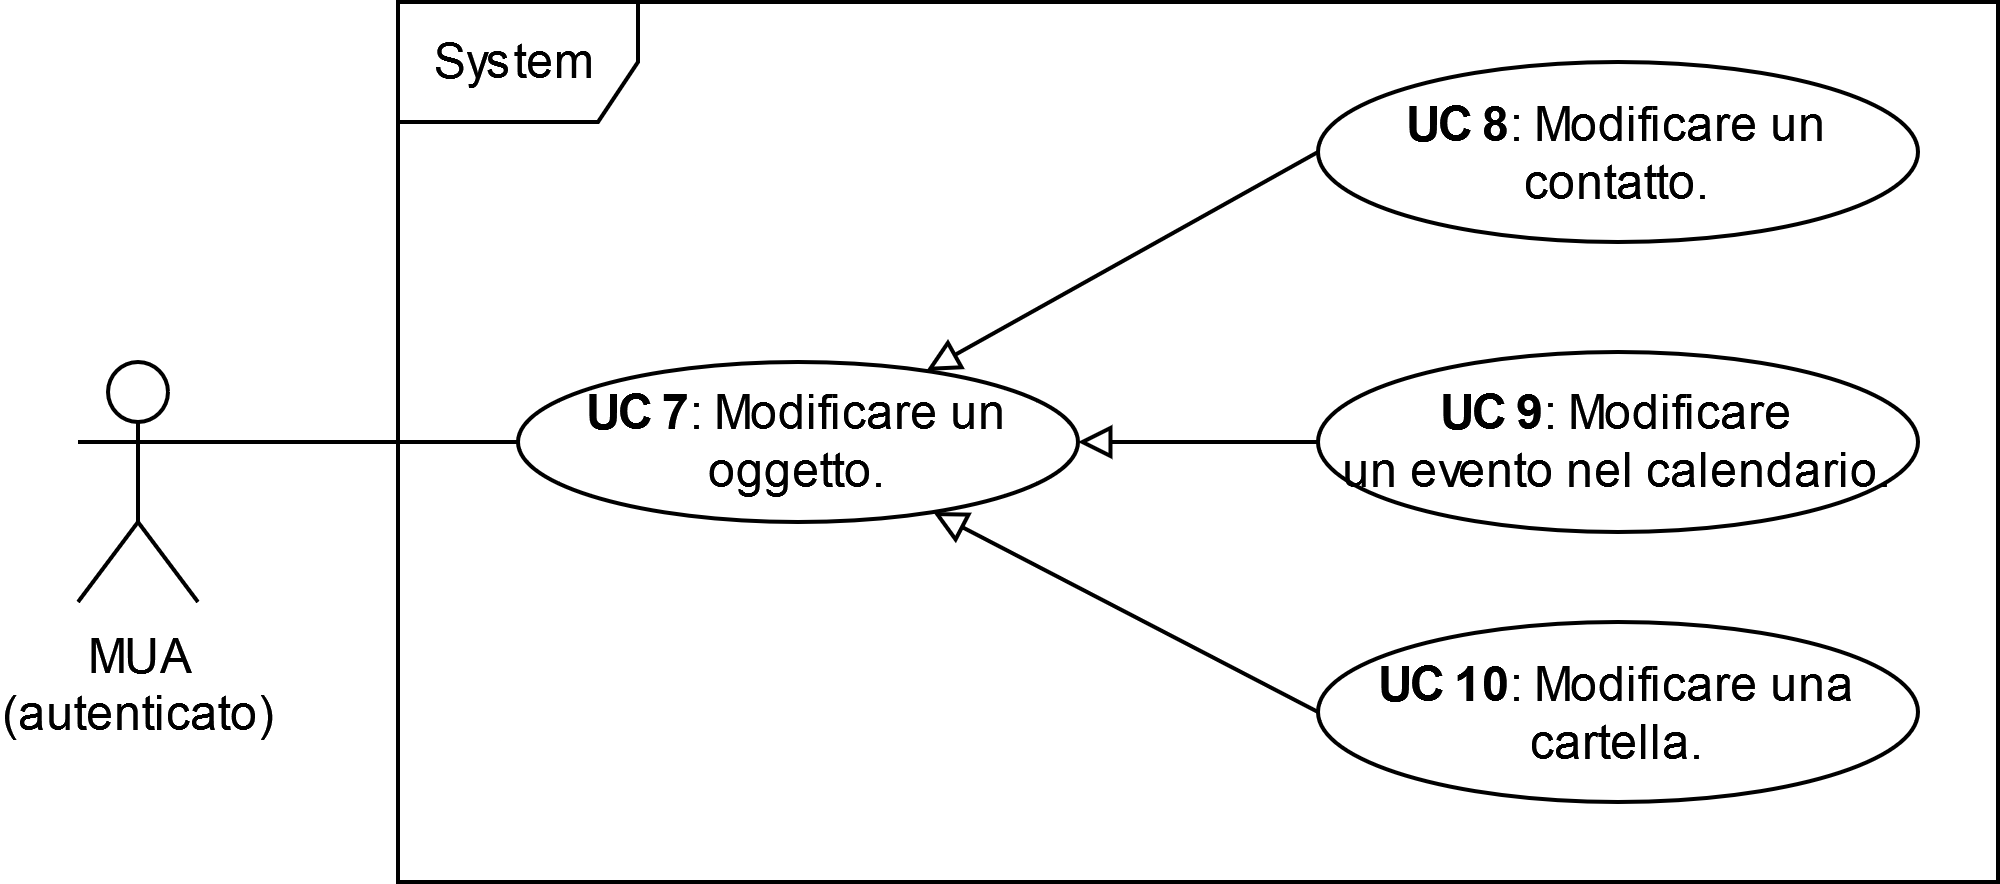
\includegraphics[width=0.85\textwidth]{sections/uc_imgs/UC07.png}
        \centering
        \caption{Diagramma sotto-casi UC 7}
    \end{figure}

    \subsubsection{UC 7.1 - Trasmette id cartella} \label{sec:UC7.1}
    \begin{itemize}
        \item \textbf{Attore principale}: MUA;
        \item \textbf{Descrizione}: il MUA trasmette l'id della cartella per condividere la cartella;
        \item \textbf{Precondizioni}: il MUA sta usando la funzionalità di creazione condivisione di una cartella;
        \item \textbf{Postcondizioni}: il sistema conosce l'id della cartella da condividere;
        \item \textbf{Scenario principale}:
            \begin{enumerate}
                \item il MUA invia l'id della cartella per condividere la cartella;
            \end{enumerate}
        \item \textbf{Inclusioni}: nessuna;
        \item \textbf{Generalizzazioni}: nessuna;
        \item \textbf{Estensioni}:
            \begin{enumerate}[label=\alph*.]
                \item il sistema non riesce a condividere la cartella perché l'id della cartella fornito non è stato trovato:
                \begin{enumerate}[label=\arabic*.]
                    \item il sistema ritorna un errore al MUA di cartella non trovata (\hyperref[sec:UC7.3]{UC 7.3}).
                \end{enumerate}
            \end{enumerate}
    \end{itemize}


    \subsubsection{UC 7.2 - Trasmette indirizzo contatto} \label{sec:UC7.2}
    \begin{itemize}
        \item \textbf{Attore principale}: MUA;
        \item \textbf{Descrizione}: il MUA trasmette l'indirizzo e-mail per la condivisione al sistema;
        \item \textbf{Precondizioni}: il MUA sta usando la funzionalità di creazione condivisione di una cartella;
        \item \textbf{Postcondizioni}: il sistema conosce l'indirizzo e-mail a cui condividere;
        \item \textbf{Scenario principale}:
            \begin{enumerate}
                \item il MUA invia l'indirizzo e-mail per la condivisione al sistema;
                \item il sistema controlla che le informazioni ricevute rispettino il seguente requisito minimo:
                    \begin{itemize}
                        \item l'indirizzo email del contatto non è una stringa vuota;
                    \end{itemize}
            \end{enumerate}
        \item \textbf{Inclusioni}: nessuna;
        \item \textbf{Generalizzazioni}: nessuna;
        \item \textbf{Estensioni}:
            \begin{enumerate}[label=\alph*.]
                \item il sistema non riesce a creare la condivisione della cartella perché l'indirizzo e-mail fornito non è valido:
                \begin{enumerate}[label=\arabic*.]
                    \item il sistema ritorna un errore al MUA di indirizzo e-mail non valido (\hyperref[sec:UC7.4]{UC 7.4}).
                \end{enumerate}
            \end{enumerate}
    \end{itemize}


\subsubsection{UC 7.3 - Ritorna errore cartella non trovata} \label{sec:UC7.3}
    \begin{itemize}
        \item \textbf{Attore principale}: MUA;
        \item \textbf{Descrizione}: il sistema non riesce a condividere la cartella perché la cartella non è stato trovato;
        \item \textbf{Precondizioni}: il MUA ha inviato l'id della cartella da condividere;
        \item \textbf{Postcondizioni}: il sistema non condivide la cartella, il MUA è stato notificato dell'errore;
        \item \textbf{Scenario principale}:
            \begin{enumerate}
                \item il sistema non trova la cartella con l'identificativo fornito dal MUA;
                \item il sistema non condivide la cartella e notifica il MUA dell'errore;
            \end{enumerate}
        \item \textbf{Inclusioni}: nessuna;
        \item \textbf{Generalizzazioni}: nessuna;
        \item \textbf{Estensioni}: nessuna.
    \end{itemize}

    \subsubsection{UC 7.4 - Ritorna errore indirizzo e-mail non valido} \label{sec:UC7.4}
    \begin{itemize}
        \item \textbf{Attore principale}: MUA;
        \item \textbf{Descrizione}: il sistema non riesce a condividere la cartella perché l'indirizzo e-mail del contatto non rispetta i requisiti;
        \item \textbf{Precondizioni}: il MUA ha inviato l'indirizzo e-mail a cui condividere;
        \item \textbf{Postcondizioni}: il sistema non condivide la cartella, il MUA è stato notificato dell'errore;
        \item \textbf{Scenario principale}:
            \begin{enumerate}
                \item il sistema controlla la sintassi dell'indirizzo e-mail e trova un errore;
                \item il sistema non condivide la cartella e notifica il MUA dell'errore;
            \end{enumerate}
        \item \textbf{Inclusioni}: nessuna;
        \item \textbf{Generalizzazioni}: nessuna;
        \item \textbf{Estensioni}: nessuna.
    \end{itemize}

    \subsection{UC 8 - Creazione condivisione contatto} \label{sec:UC8}

    \begin{itemize}
        \item \textbf{Attore principale}: MUA;
        \item \textbf{Descrizione}: il MUA deve poter creare una condivisione di un contatto nel sistema;
        \item \textbf{Precondizioni}: il MUA sta usando la funzionalità di creazione di una condivisione;
        \item \textbf{Postcondizioni}: il sistema condivide il contatto con l'indirizzo e-mail fornito dal MUA;
        \item \textbf{Scenario principale}:
            \begin{enumerate}
                \item il MUA trasmette l'id del contatto da condividere (\hyperref[sec:UC8.1]{UC 8.1});
                \item il MUA trasmette l'indirizzo e-mail a cui condividere (\hyperref[sec:UC8.2]{UC 8.2});
                \item il sistema condivide il contatto.
            \end{enumerate}
        \item \textbf{Inclusioni}: nessuna;
        \item \textbf{Generalizzazioni}: nessuna;
        \item \textbf{Estensioni}: nessuna.
    \end{itemize}


    \begin{figure}[H]
        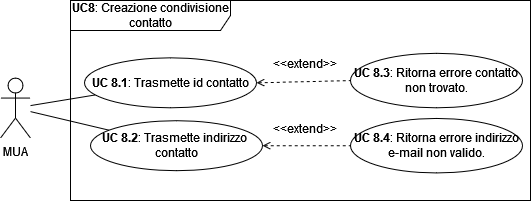
\includegraphics[width=0.85\textwidth]{sections/uc_imgs/UC08.png}
        \centering
        \caption{Diagramma sotto-casi UC 8}
    \end{figure}

    \subsubsection{UC 8.1 - Trasmette id contatto} \label{sec:UC8.1}
    \begin{itemize}
        \item \textbf{Attore principale}: MUA;
        \item \textbf{Descrizione}: il MUA trasmette l'id del contatto per identificare il contatto da condividere;
        \item \textbf{Precondizioni}: il MUA sta usando la funzionalità di creazione condivisione di un contatto;
        \item \textbf{Postcondizioni}: il sistema conosce l'id del contatto da condividere;
        \item \textbf{Scenario principale}:
            \begin{enumerate}
                \item il MUA invia l'id del contatto per condividere il contatto.
            \end{enumerate}
        \item \textbf{Inclusioni}: nessuna;
        \item \textbf{Generalizzazioni}: nessuna;
        \item \textbf{Estensioni}:
            \begin{enumerate}[label=\alph*.]
                \item il sistema non riesce a condividere il contatto perché l'id del contatto fornito non è stato trovato:
                \begin{enumerate}[label=\arabic*.]
                    \item il sistema ritorna un errore al MUA di contatto non trovato (\hyperref[sec:UC8.3]{UC 8.3}).
                \end{enumerate}
            \end{enumerate}
    \end{itemize}


    \subsubsection{UC 8.2 - Trasmette indirizzo contatto} \label{sec:UC8.2}
    \begin{itemize}
        \item \textbf{Attore principale}: MUA;
        \item \textbf{Descrizione}: il MUA trasmette l'indirizzo e-mail per la condivisione al sistema;
        \item \textbf{Precondizioni}: il MUA sta usando la funzionalità di creazione condivisione di un contatto;
        \item \textbf{Postcondizioni}: il sistema conosce l'indirizzo e-mail a cui condividere;
        \item \textbf{Scenario principale}:
            \begin{enumerate}
                \item il MUA invia l'indirizzo e-mail per la condivisione al sistema;
                \item il sistema controlla che le informazioni ricevute rispettino il seguente requisito minimo:
                    \begin{itemize}
                        \item l'indirizzo e-mail del contatto non è una stringa vuota.
                    \end{itemize}
            \end{enumerate}
        \item \textbf{Inclusioni}: nessuna;
        \item \textbf{Generalizzazioni}: nessuna;
        \item \textbf{Estensioni}:
            \begin{enumerate}[label=\alph*.]
                \item il sistema non riesce a creare la condivisione del contatto perché l'indirizzo e-mail fornito non è valido:
                \begin{enumerate}[label=\arabic*.]
                    \item il sistema ritorna un errore al MUA di indirizzo e-mail non valido (\hyperref[sec:UC8.4]{UC 8.4}).
                \end{enumerate}
            \end{enumerate}
    \end{itemize}


\subsubsection{UC 8.3 - Ritorna errore contatto non trovato} \label{sec:UC8.3}
    \begin{itemize}
        \item \textbf{Attore principale}: MUA;
        \item \textbf{Descrizione}: il sistema non riesce a condividere il contatto perché il contatto non è stato trovato;
        \item \textbf{Precondizioni}: il MUA ha inviato l'id del contatto da condividere;
        \item \textbf{Postcondizioni}: il sistema non condivide il contatto, il MUA è stato notificato dell'errore;
        \item \textbf{Scenario principale}:
            \begin{enumerate}
                \item il sistema non trova il contatto con l'identificativo fornito dal MUA;
                \item il sistema non condivide il contatto e notifica il MUA dell'errore.
            \end{enumerate}
        \item \textbf{Inclusioni}: nessuna;
        \item \textbf{Generalizzazioni}: nessuna;
        \item \textbf{Estensioni}: nessuna.
    \end{itemize}

\subsubsection{UC 8.4 - Ritorna errore indirizzo e-mail non valido} \label{sec:UC8.4}
    \begin{itemize}
        \item \textbf{Attore principale}: MUA;
        \item \textbf{Descrizione}: il sistema non riesce a condividere il contatto perché l'indirizzo e-mail del contatto non rispetta i requisiti;
        \item \textbf{Precondizioni}: il MUA ha inviato l'indirizzo e-mail a cui condividere;
        \item \textbf{Postcondizioni}: il sistema non condivide il contatto, il MUA è stato notificato dell'errore;
        \item \textbf{Scenario principale}:
            \begin{enumerate}
                \item il sistema controlla la sintassi dell'indirizzo e-mail e trova un errore;
                \item il sistema non condivide il contatto e notifica il MUA dell'errore.
            \end{enumerate}
        \item \textbf{Inclusioni}: nessuna;
        \item \textbf{Generalizzazioni}: nessuna;
        \item \textbf{Estensioni}: nessuna.
    \end{itemize}




    %LTeX: language=it
\subsection{UC 11 - Eliminare un oggetto} \label{sec:UC3}
    \begin{figure}[h]
        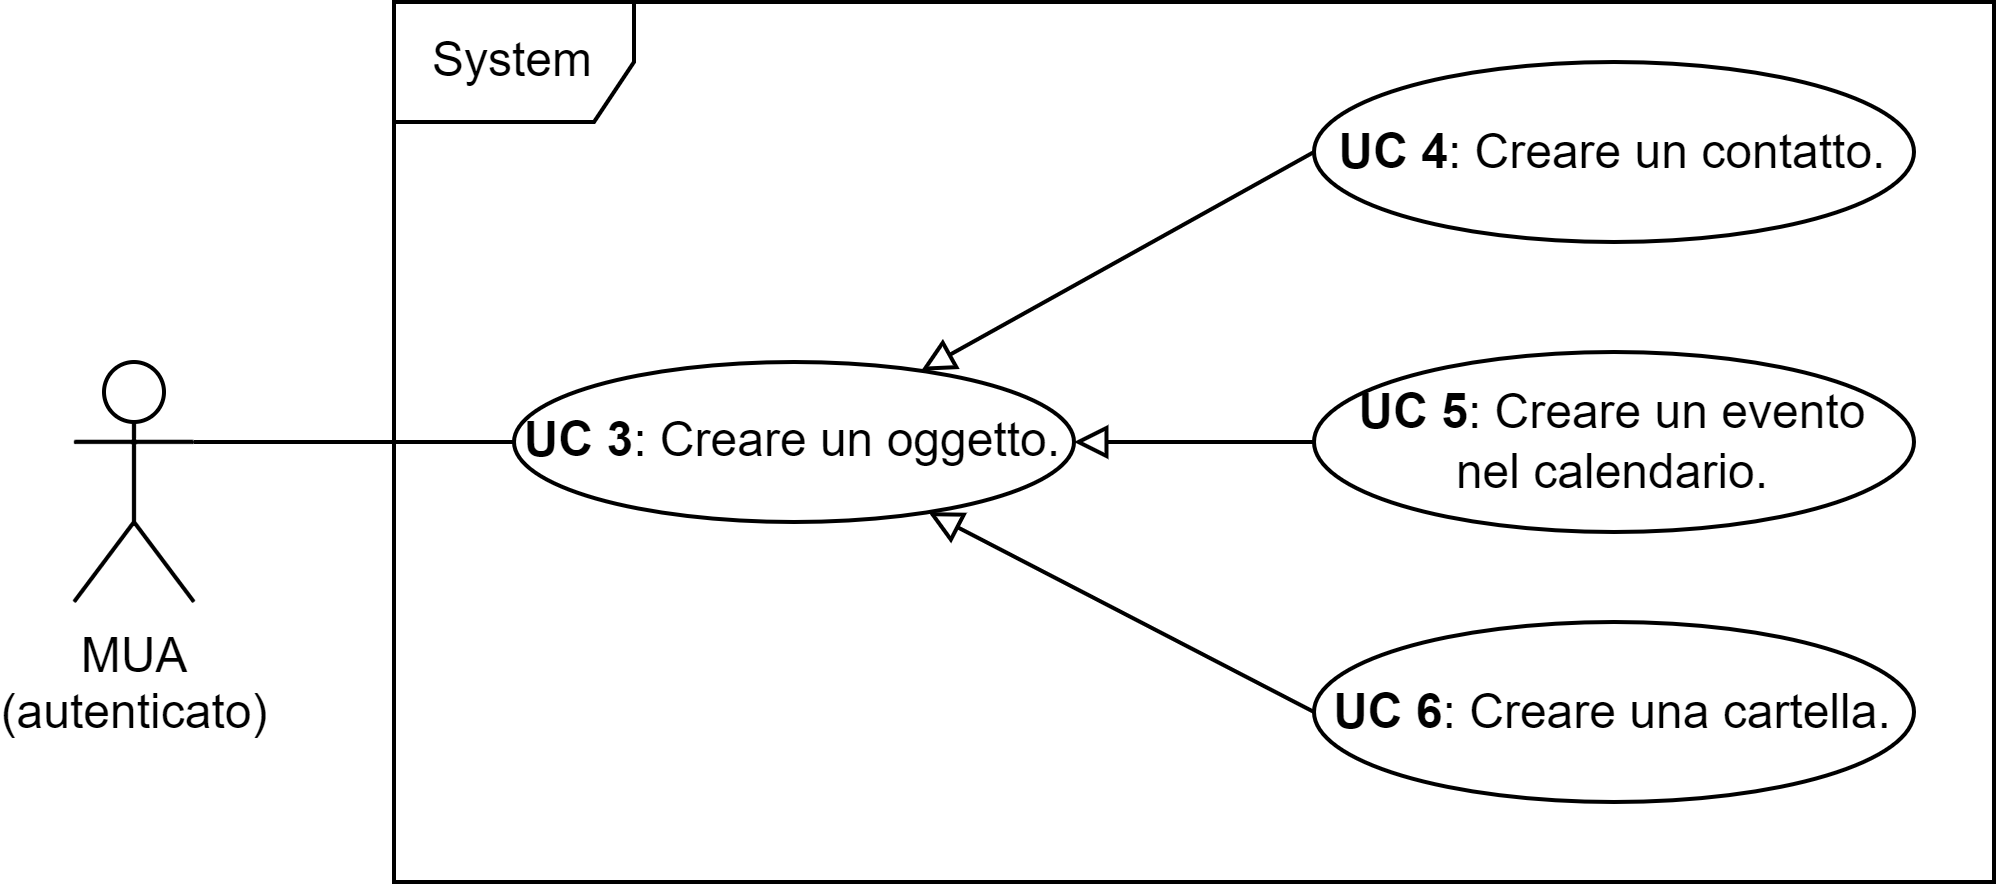
\includegraphics[width=0.85\textwidth]{sections/uc_imgs/UC03.png}
        \centering
        \caption{Diagramma UC11 }
    \end{figure}
    \begin{itemize}
        \item \textbf{Attore principale}: MUA;
        \item \textbf{Descrizione}: il MUA deve poter eliminare un oggetto dal sistema;
        \item \textbf{Precondizioni}: l’account che il MUA gestisce è registrato nel sistema, e ha un connessione aperta con il sistema ed è autenticato;
        \item \textbf{Postcondizioni}: il MUA elimina un oggetto che è stato rimosso dal sistema;
        \item \textbf{Scenario principale}:
            \begin{enumerate}
                \item il MUA invia i dettagli necessari ad indentificare l'oggetto da eliminare al sistema;
                \item il sistema elimina l'oggetto;
            \end{enumerate}
        \item \textbf{Inclusioni}: nessuna;
        \item \textbf{Generalizzazioni}:
            \begin{itemize}
                \item il MUA elimina un contatto (\hyperref[sec:UC12]{UC 12});
                \item il MUA elimina un evento nel calendario (\hyperref[sec:UC13]{UC 13});
                \item il MUA elimina una cartella (\hyperref[sec:UC14]{UC 14});
            \end{itemize}
        \item \textbf{Estensioni}: 
        \begin{itemize}
            \item 
        \end{itemize}
    \end{itemize}

    %     \subsection{UC 3 - Creare un oggetto} \label{sec: UC 3}
%     \begin{itemize}
%         \item Attore: MUA;
%         \item Descrizione: il MUA deve poter creare un oggetto specifico;
%         \item Scenario principale:
%             \begin{enumerate}
%                 \item 
%             \end{enumerate}
%         \item Generalizzazioni:
%             \begin{itemize}
%                 \item il MUA crea una cartella (\hyperref[sec: UC 3.1]{UC 3.1});
%                 \item il MUA crea un contatto (\hyperref[sec: UC 3.2]{UC 3.2});
%                 \item il MUA crea una condivisione (\hyperref[sec: UC 3.3]{UC 3.3});
%                 \item il MUA crea un evento (\hyperref[sec: UC 3.4]{UC 3.4}).
%             \end{itemize}
%         \item Estensioni: errore ;
%         \item Precondizioni: l’account che il MUA gestisce è registrato nel sistema ed è autenticato;
%         \item Postcondizioni: è stato creato l’oggetto desiderato.
%     \end{itemize}
    %LTeX: language=it
\subsection{UC 12 - Modifica contatto} \label{sec:UC12}
    \begin{itemize}
        \item \textbf{Attore principale}: MUA;
        \item \textbf{Descrizione}: il MUA deve poter modificare un contatto nel sistema;
        \item \textbf{Precondizioni}: l’account che il MUA gestisce è registrato nel sistema, ha una connessione aperta con il sistema ed è autenticato;
        \item \textbf{Postcondizioni}: il contatto è stata modificato con successo, ed è stato salvato nel sistema
        \item \textbf{Scenario principale}:
            \begin{enumerate}
                \item il MUA trasmette il nuovo nome del contatto (\hyperref[sec:UC12.1]{UC 12.1});
                \item il MUA trasmette il nuovo indirizzo e-mail del contatto (\hyperref[sec:UC12.2]{UC 12.2});
                \item il sistema salva il contatto modificato;
            \end{enumerate}
        \item \textbf{Inclusioni}: nessuna;
        \item \textbf{Generalizzazioni}: nessuna;
        \item \textbf{Estensioni}: nessuna.
    \end{itemize}

\begin{figure}[h]
    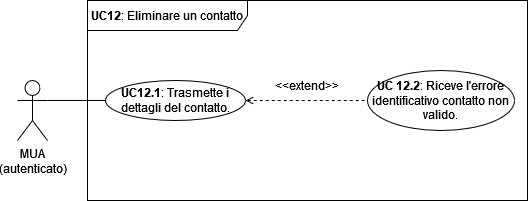
\includegraphics[width=0.85\textwidth]{sections/uc_imgs/UC12.png}
    \centering
    \caption{Diagramma sotto-casi UC 12}
\end{figure}

\subsubsection{UC 12.1 - Trasmette nome contatto} \label{sec:UC12.1}
    \begin{itemize}
        \item \textbf{Attore principale}: MUA;
        \item \textbf{Descrizione}: il MUA trasmette il nuovo nome per modificare il contatto al sistema;
        \item \textbf{Precondizioni}: il MUA sta usando la funzionalità di modifica di un contatto;
        \item \textbf{Postcondizioni}: il sistema conosce il nuovo nome del contatto;
        \item \textbf{Scenario principale}:
            \begin{enumerate}
                \item il MUA invia il nuovo nome per modificare il contatto al sistema;
                \item il sistema controlla che le informazioni ricevute rispettino il seguente requisito minimo:
                    \begin{itemize}
                        \item il nome del contatto non è una stringa vuota;
                    \end{itemize}
            \end{enumerate}
        \item \textbf{Inclusioni}: nessuna;
        \item \textbf{Generalizzazioni}: nessuna;
        \item \textbf{Estensioni}:
            \begin{enumerate}[label=\alph*.]
                \item il sistema non riesce a modificare il contatto perché il nome fornito non è valido:
                \begin{enumerate}[label=\arabic*.]
                    \item il sistema ritorna un errore al MUA di nome non valido (\hyperref[sec:UC12.3]{UC 12.3}).
                \end{enumerate}
            \end{enumerate}
    \end{itemize}


    \subsubsection{UC 12.2 - Trasmette l'indirizzo e-mail del contatto} \label{sec:UC12.2}
    \begin{itemize}
        \item \textbf{Attore principale}: MUA;
        \item \textbf{Descrizione}: il MUA trasmette il nuovo indirizzo e-mail per modificare il contatto al sistema;
        \item \textbf{Precondizioni}: il MUA sta usando la funzionalità di modifica di un contatto;
        \item \textbf{Postcondizioni}: il sistema conosce il nuovo indirizzo e-mail del contatto;
        \item \textbf{Scenario principale}:
            \begin{enumerate}
                \item il MUA invia il nuovo indirizzo e-mail per modificare il contatto al sistema;
                \item il sistema controlla che le informazioni ricevute rispettino il seguente requisito minimo:
                    \begin{itemize}
                        \item l'indirizzo e-mail del contatto non è una stringa vuota;
                    \end{itemize}
            \end{enumerate}
        \item \textbf{Inclusioni}: nessuna;
        \item \textbf{Generalizzazioni}: nessuna;
        \item \textbf{Estensioni}:
            \begin{enumerate}[label=\alph*.]
                \item il sistema non riesce a modificare il contatto perché l'indirizzo e-mail fornito non è valido:
                \begin{enumerate}[label=\arabic*.]
                    \item il sistema ritorna un errore al MUA di indirizzo e-mail non valido (\hyperref[sec:UC12.4]{UC 12.4}).
                \end{enumerate}
            \end{enumerate}
    \end{itemize}


\subsubsection{UC 12.3 - Ritorna l'errore nome non valido} \label{sec:UC12.3}
    \begin{itemize}
        \item \textbf{Attore principale}: MUA;
        \item \textbf{Descrizione}: il sistema non riesce a modificare il contatto perché il nome del contatto non rispetta i requisiti;
        \item \textbf{Precondizioni}: il MUA ha inviato il nome del contatto;
        \item \textbf{Postcondizioni}: il sistema non modifica il contatto, il MUA è stato notificato dell'errore;
        \item \textbf{Scenario principale}:
            \begin{enumerate}
                \item il sistema controlla la sintassi del nome del contatto e trova un errore;
                \item il sistema non modifica il contatto e notifica il MUA dell'errore;
            \end{enumerate}
        \item \textbf{Inclusioni}: nessuna;
        \item \textbf{Generalizzazioni}: nessuna;
        \item \textbf{Estensioni}: nessuna.
    \end{itemize}

\subsubsection{UC 12.4 - Ritorna l'errore indirizzo e-mail non valido} \label{sec:UC12.4}
    \begin{itemize}
        \item \textbf{Attore principale}: MUA;
        \item \textbf{Descrizione}: il sistema non riesce a modificare il contatto perché l'indirizzo e-mail del contatto non rispetta i requisiti;
        \item \textbf{Precondizioni}: il MUA ha inviato l'indirizzo e-mail del contatto;
        \item \textbf{Postcondizioni}: il sistema non modifica il contatto, il MUA è stato notificato dell'errore;
        \item \textbf{Scenario principale}:
            \begin{enumerate}
                \item il sistema controlla la sintassi dell'indirizzo e-mail del contatto e trova un errore;
                \item il sistema non modifica il contatto e notifica il MUA dell'errore;
            \end{enumerate}
        \item \textbf{Inclusioni}: nessuna;
        \item \textbf{Generalizzazioni}: nessuna;
        \item \textbf{Estensioni}: nessuna.
    \end{itemize}
    %LTeX: language=it
\subsection{UC 13 - Modifica evento} \label{sec:UC13}
    \begin{itemize}
        \item \textbf{Attore principale}: MUA;
        \item \textbf{Descrizione}: il MUA deve poter modificare un evento nel sistema;
        \item \textbf{Precondizioni}: l’account che il MUA gestisce è registrato nel sistema, ha una connessione aperta con il sistema ed è autenticato;
        \item \textbf{Postcondizioni}: il MUA modifica l'evento che viene salvato nel sistema;
        \item \textbf{Scenario principale}:
            \begin{enumerate}
                \item il MUA trasmette il nuovo titolo dell'evento (\hyperref[sec:UC13.1]{UC 13.1});
                \item il MUA trasmette la nuova data di inizio dell'evento (\hyperref[sec:UC13.2]{UC 13.2});
                \item il MUA trasmette la nuova data di fine dell'evento (\hyperref[sec:UC13.3]{UC 13.3});
                \item il MUA trasmette la nuova durata dell'evento (\hyperref[sec:UC13.4]{UC 13.4});
                \item il sistema salva l'evento.
            \end{enumerate}
        \item \textbf{Inclusioni}: nessuna;
        \item \textbf{Generalizzazioni}: nessuna;
        \item \textbf{Estensioni}: nessuna.
    \end{itemize}

\begin{figure}[H]
    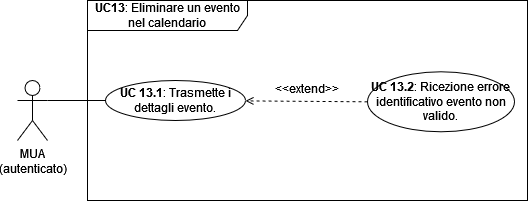
\includegraphics[width=0.813\textwidth]{sections/uc_imgs/UC13.png}
    \centering
    \caption{Diagramma sotto-casi UC 13}
\end{figure}

\subsubsection{UC 13.1 - Trasmette titolo evento} \label{sec:UC13.1}
    \begin{itemize}
        \item \textbf{Attore principale}: MUA;
        \item \textbf{Descrizione}: il MUA trasmette il nuovo titolo per modificare l'evento al sistema;
        \item \textbf{Precondizioni}: il MUA sta usando la funzionalità di modifica di un evento;
        \item \textbf{Postcondizioni}: il sistema conosce il nuovo titolo dell'evento;
        \item \textbf{Scenario principale}:
            \begin{enumerate}
                \item il MUA invia il nuovo titolo per modificare l'evento al sistema;
                \item il sistema controlla che le informazioni ricevute rispettino il seguente requisito minimo:
                    \begin{itemize}
                        \item il titolo dell'evento non è una stringa vuota.
                    \end{itemize}
            \end{enumerate}
        \item \textbf{Inclusioni}: nessuna;
        \item \textbf{Generalizzazioni}: nessuna;
        \item \textbf{Estensioni}:
            \begin{enumerate}[label=\alph*.]
                \item il sistema non riesce a modificare l'evento perché il titolo fornito non è valido:
                \begin{enumerate}[label=\arabic*.]
                    \item il sistema ritorna un errore al MUA di titolo evento non valido (\hyperref[sec:UC13.5]{UC 13.5}).
                \end{enumerate}
            \end{enumerate}
    \end{itemize}



    \subsubsection{UC 13.2 - Trasmette data inizio evento} \label{sec:UC13.2}
    \begin{itemize}
        \item \textbf{Attore principale}: MUA;
        \item \textbf{Descrizione}: il MUA trasmette la nuova data di inizio dell'evento per modificare l'evento al sistema;
        \item \textbf{Precondizioni}: il MUA sta usando la funzionalità di modifica di un evento;
        \item \textbf{Postcondizioni}: il sistema conosce la nuova data di inizio dell'evento;
        \item \textbf{Scenario principale}:
            \begin{enumerate}
                \item il MUA invia la nuova data di inizio dell'evento per modificare l'evento al sistema;
                \item il sistema controlla che le informazioni ricevute rispettino il seguente requisito minimo:
                    \begin{itemize}
                        \item la data di inizio dell'evento è in un formato corretto.
                    \end{itemize}
            \end{enumerate}
        \item \textbf{Inclusioni}: nessuna;
        \item \textbf{Generalizzazioni}: nessuna;
        \item \textbf{Estensioni}:
            \begin{enumerate}[label=\alph*.]
                \item il sistema non riesce a modificare l'evento perché la data di inizio dell'evento fornita non è in un formato corretto:
                \begin{enumerate}[label=\arabic*.]
                    \item il sistema ritorna un errore al MUA di data evento non valida (\hyperref[sec:UC13.6]{UC 13.6}).
                \end{enumerate}
            \end{enumerate}
    \end{itemize}


    \subsubsection{UC 13.3 - Trasmette data fine evento} \label{sec:UC13.3}
    \begin{itemize}
        \item \textbf{Attore principale}: MUA;
        \item \textbf{Descrizione}: il MUA trasmette la nuova data di fine dell'evento per modificare l'evento al sistema;
        \item \textbf{Precondizioni}: il MUA sta usando la funzionalità di modifica di un evento;
        \item \textbf{Postcondizioni}: il sistema conosce la nuova data di fine dell'evento;
        \item \textbf{Scenario principale}:
            \begin{enumerate}
                \item il MUA invia la nuova data di fine dell'evento per modificare l'evento al sistema;
                \item il sistema controlla che le informazioni ricevute rispettino il seguente requisito minimo:
                    \begin{itemize}
                        \item la data di fine dell'evento è in un formato corretto.
                    \end{itemize}
            \end{enumerate}
        \item \textbf{Inclusioni}: nessuna;
        \item \textbf{Generalizzazioni}: nessuna;
        \item \textbf{Estensioni}:
            \begin{enumerate}[label=\alph*.]
                \item il sistema non riesce a modificare l'evento perché la data di fine dell'evento fornita non è in un formato corretto:
                \begin{enumerate}[label=\arabic*.]
                    \item il sistema ritorna un errore al MUA di data evento non valida (\hyperref[sec:UC13.6]{UC 13.6}).
                \end{enumerate}
            \end{enumerate}
    \end{itemize}

    \subsubsection{UC 13.4 - Trasmette durata evento} \label{sec:UC13.4}
    \begin{itemize}
        \item \textbf{Attore principale}: MUA;
        \item \textbf{Descrizione}: il MUA trasmette la nuova durata per modificare l'evento al sistema;
        \item \textbf{Precondizioni}: il MUA sta usando la funzionalità di modifica di un evento;
        \item \textbf{Postcondizioni}: il sistema conosce la nuova durata dell'evento;
        \item \textbf{Scenario principale}:
            \begin{enumerate}
                \item il MUA invia la nuova durata per modificare l'evento al sistema;
                \item il sistema controlla che le informazioni ricevute rispettino il seguente requisito minimo:
                    \begin{itemize}
                        \item la durata dell'evento deve essere consistente con la data di inizio e la data di fine.
                    \end{itemize}
            \end{enumerate}
        \item \textbf{Inclusioni}: nessuna;
        \item \textbf{Generalizzazioni}: nessuna;
        \item \textbf{Estensioni}:
            \begin{enumerate}[label=\alph*.]
                \item il sistema non riesce a modificare l'evento perché la durata fornita non è valida:
                \begin{enumerate}[label=\arabic*.]
                    \item il sistema ritorna un errore al MUA di durata inconsistente (\hyperref[sec:UC13.7]{UC 13.7}).
                \end{enumerate}
            \end{enumerate}
    \end{itemize}


    \subsubsection{UC 13.5 - Ritorna errore titolo evento non valido} \label{sec:UC13.5}
    \begin{itemize}
        \item \textbf{Attore principale}: MUA;
        \item \textbf{Descrizione}: il sistema non riesce a modificare l'evento perché il titolo dell'evento non rispetta i requisiti;
        \item \textbf{Precondizioni}: il MUA ha inviato il titolo dell'evento;
        \item \textbf{Postcondizioni}: il sistema non modifica l'evento, il MUA è stato notificato dell'errore;
        \item \textbf{Scenario principale}:
            \begin{enumerate}
                \item il sistema controlla la sintassi del titolo dell'evento e trova un errore;
                \item il sistema non modifica l'evento e notifica il MUA dell'errore.
            \end{enumerate}
        \item \textbf{Inclusioni}: nessuna;
        \item \textbf{Generalizzazioni}: nessuna;
        \item \textbf{Estensioni}: nessuna.
    \end{itemize}


    \subsubsection{UC 13.6 - Ritorna errore data non valida} \label{sec:UC13.6}
    \begin{itemize}
        \item \textbf{Attore principale}: MUA;
        \item \textbf{Descrizione}: il sistema non riesce a modificare l'evento perché la data non è nel formato corretto;
        \item \textbf{Precondizioni}: il MUA ha inviato la data dell'evento;
        \item \textbf{Postcondizioni}: il sistema non modifica l'evento, il MUA è stato notificato dell'errore;
        \item \textbf{Scenario principale}:
            \begin{enumerate}
                \item il sistema controlla il formato della data dell'evento e trova un errore;
                \item il sistema non salva l'evento e notifica il MUA dell'errore.
            \end{enumerate}
        \item \textbf{Inclusioni}: nessuna;
        \item \textbf{Generalizzazioni}: nessuna;
        \item \textbf{Estensioni}: nessuna.
    \end{itemize}

    \subsubsection{UC 13.7 - Ritorna errore durata inconsistente} \label{sec:UC13.7}
    \begin{itemize}
        \item \textbf{Attore principale}: MUA;
        \item \textbf{Descrizione}: il sistema non riesce a modificare l'evento perché la durata non rispetta i requisiti;
        \item \textbf{Precondizioni}: il MUA ha inviato la durata dell'evento;
        \item \textbf{Postcondizioni}: il sistema non modifica l'evento, il MUA è stato notificato dell'errore;
        \item \textbf{Scenario principale}:
            \begin{enumerate}
                \item il sistema controlla la consistenza della durata e trova un errore;
                \item il sistema non modifica l'evento e notifica il MUA dell'errore.
            \end{enumerate}
        \item \textbf{Inclusioni}: nessuna;
        \item \textbf{Generalizzazioni}: nessuna;
        \item \textbf{Estensioni}: nessuna.
    \end{itemize}
    \subsubsection{UC 14 - Eliminare una cartella} \label{sec:UC14}
    \begin{itemize}
        \item \textbf{Attore principale}: MUA;
        \item \textbf{Descrizione}: il MUA elimina una cartella dal sistema;
        \item \textbf{Precondizioni}: il MUA sta usando la funzionalità di eliminazione di un oggetto;
        \item \textbf{Postcondizioni}: il sistema elimina la cartella con l'identificativo fornito dal MUA;
        \item \textbf{Scenario principale}:
            \begin{enumerate}
                \item il MUA invia i dettagli della cartella da eliminare al sistema (\hyperref[sec:UC14.1]{UC 14.1});
                \item il sistema elimina la cartella;
            \end{enumerate}
        \item \textbf{Inclusioni}: nessuna;
        \item \textbf{Generalizzazioni}: nessuna;
        \item \textbf{Estensioni}: nessuna.
    \end{itemize}

\begin{figure}[h]
    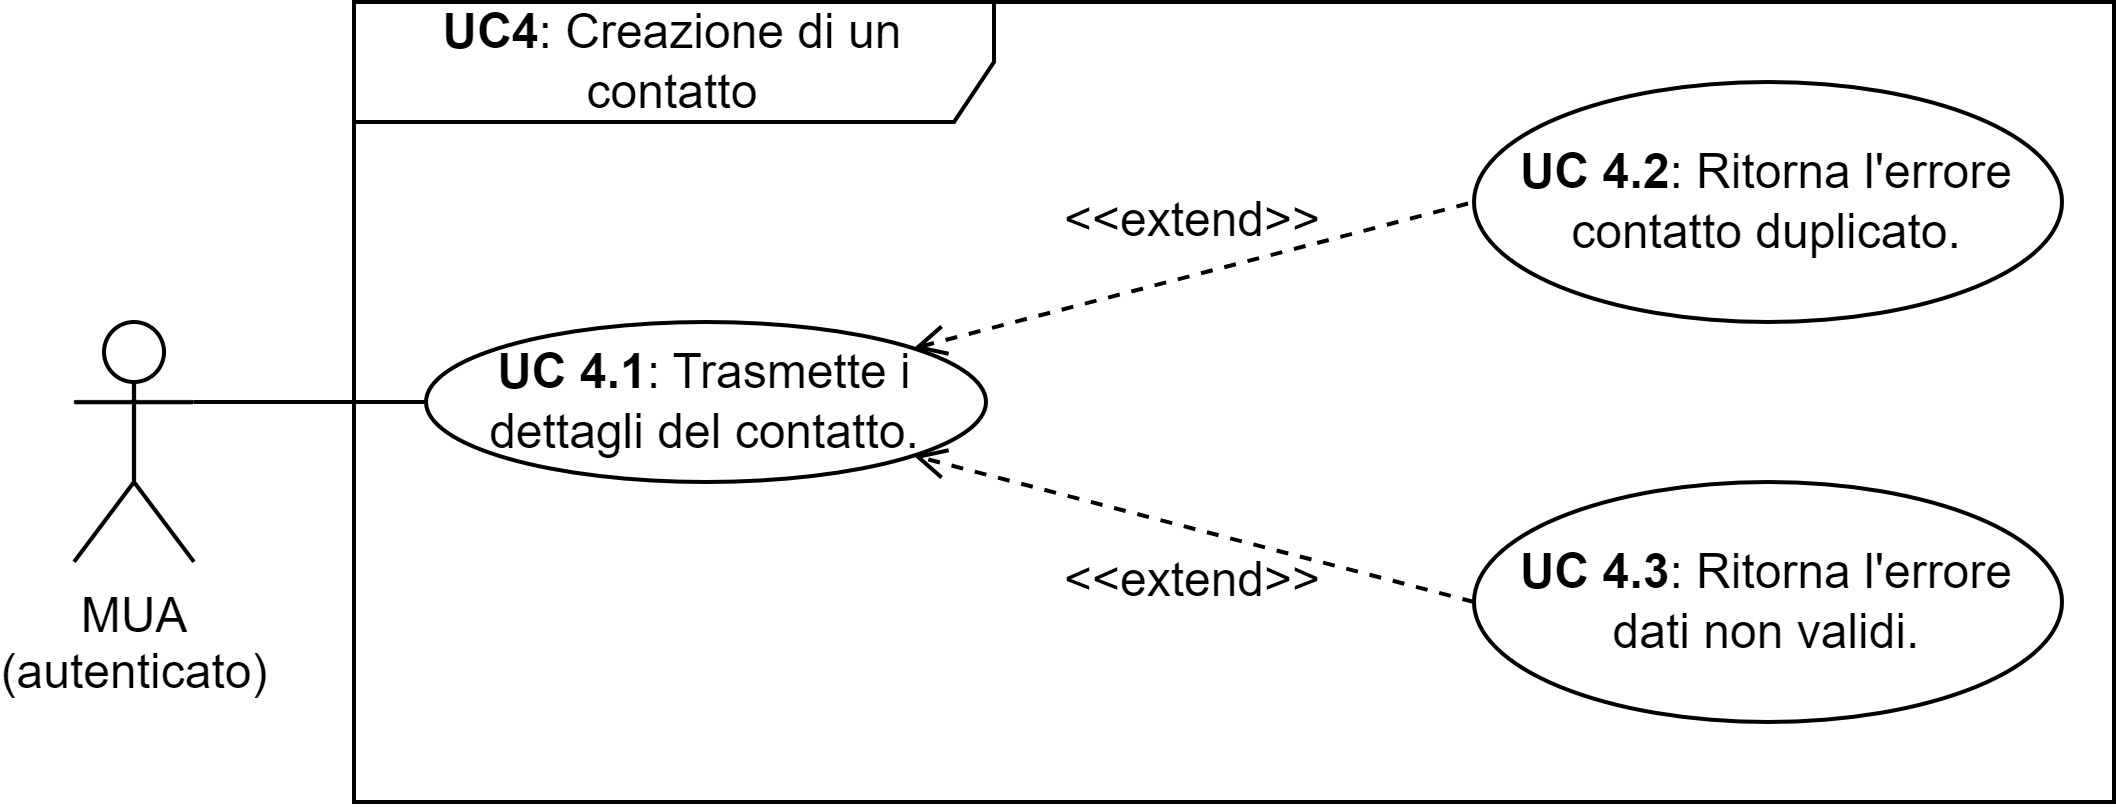
\includegraphics[width=0.85\textwidth]{sections/uc_imgs/UC04.X.png}
    \centering
    \caption{Diagramma sotto-casi UC 14.}
\end{figure}

\subsubsection{UC 14.1 - Trasmette i dettagli della cartella} \label{sec:UC14.1}
    \begin{figure}[h]
        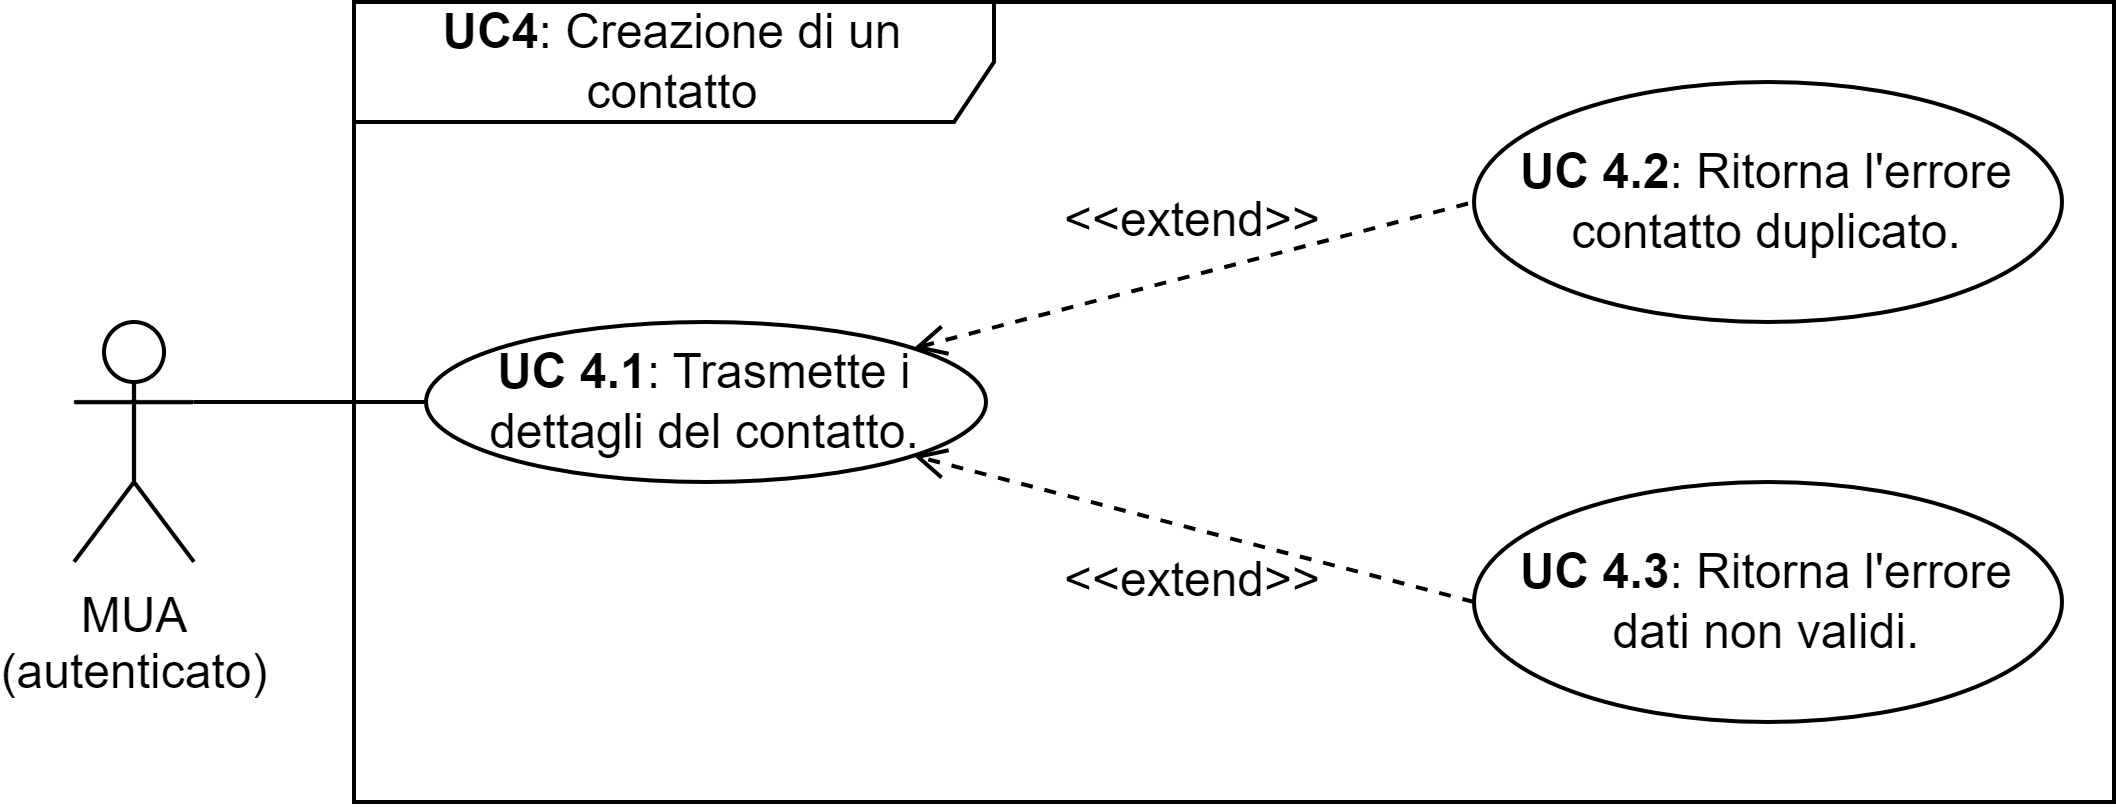
\includegraphics[width=0.85\textwidth]{sections/uc_imgs/UC04.X.png}
        \centering
        \caption{Diagramma UC 14.1.}
    \end{figure}
    \begin{itemize}
        \item \textbf{Attore principale}: MUA;
        \item \textbf{Descrizione}: il MUA invia le informazioni della cartella da eliminare al sistema;
        \item \textbf{Precondizioni}: il MUA sta usando la funzionalità di eliminazione di una cartella;
        \item \textbf{Postcondizioni}: il sistema elimina la cartella identificata dalle informazioni fornite dal MUA;
        \item \textbf{Scenario principale}:
            \begin{enumerate}
                \item il MUA invia l'identificativo della cartella al sistema;
                \item il sistema controlla che la cartella identificata rispetti i seguenti requisiti:
                \begin{itemize}
                    \item la cartella non contiene altre email;
                    \item la cartella non contiene altre cartelle;
                \end{itemize}
            \end{enumerate}
        \item \textbf{Inclusioni}: nessuna;
        \item \textbf{Generalizzazioni}: nessuna;
        \item \textbf{Estensioni}:
            \begin{enumerate}[label=\alph*.]
                \item il sistema non riesce a eliminare la cartella perché non è stata trovata:
                \begin{enumerate}[label=\arabic*.]
                    \item il sistema ritorna un errore al MUA di identificativo non valido (\hyperref[sec:UC14.2]{UC 14.2}).
                \end{enumerate}
                \item il sistema non riesce a eliminare la cartella perché contiene delle email:
                \begin{enumerate}[label=\arabic*.]
                    \item il sistema ritorna un errore al MUA di cartella contenente email (\hyperref[sec:UC14.3]{UC 14.3}).
                \end{enumerate}
                \item il sistema non riesce a eliminare la cartella perché contiene altre cartelle:
                \begin{enumerate}[label=\arabic*.]
                    \item il sistema ritorna un errore al MUA di cartella contenente cartelle (\hyperref[sec:UC14.4]{UC 14.4}).
                \end{enumerate}
            \end{enumerate}
    \end{itemize}


\subsubsection{UC 14.2 - Ricezione errore identificativo cartella non valida} \label{sec:UC14.2}
    \begin{itemize}
        \item \textbf{Attore principale}: MUA;
        \item \textbf{Descrizione}: il sistema non riesce a eliminare la cartella perché l'identificativo cartella non è stato trovato;
        \item \textbf{Precondizioni}: il MUA sta usando la funzionalità d'invio dei dettagli al sistema di una cartella;
        \item \textbf{Postcondizioni}: il sistema non elimina la cartella, il MUA è stato notificato dell'errore;
        \item \textbf{Scenario principale}:
            \begin{enumerate}
                \item il sistema non trova la cartella con l'identificativo fornito dal MUA;
                \item il sistema non elimina la cartella e notifica il MUA dell'errore;
            \end{enumerate}
        \item \textbf{Inclusioni}: nessuna;
        \item \textbf{Generalizzazioni}: nessuna;
        \item \textbf{Estensioni}: nessuna.
    \end{itemize}
   
    \subsubsection{UC 14.3 - Ricezione errore cartella contenente email} \label{sec:UC14.3}

    \begin{itemize}
        \item \textbf{Attore principale}: MUA;
        \item \textbf{Descrizione}: il sistema non riesce a eliminare la cartella perché una o più email sono presenti all'interno di quella cartella;
        \item \textbf{Precondizioni}: il MUA sta usando la funzionalità d'invio dei dettagli al sistema di una cartella;
        \item \textbf{Postcondizioni}: il sistema non elimina la cartella, il MUA è stato notificato dell'errore;
        \item \textbf{Scenario principale}:
            \begin{enumerate}
                \item la cartella non soddisfa il requisito di non conetenere email;
                \item il sistema non elimina la cartella e notifica il MUA dell'errore;
            \end{enumerate}
        \item \textbf{Inclusioni}: nessuna;
        \item \textbf{Generalizzazioni}: nessuna;
        \item \textbf{Estensioni}: nessuna.
    \end{itemize}


    \subsubsection{UC 14.4 - Ricezione errore cartella contenente cartelle} \label{sec:UC14.4}

    \begin{itemize}
        \item \textbf{Attore principale}: MUA;
        \item \textbf{Descrizione}: il sistema non riesce a eliminare la cartella perché una o più cartelle sono presenti all'interno di quella cartella;
        \item \textbf{Precondizioni}: il MUA sta usando la funzionalità d'invio dei dettagli al sistema di una cartella;
        \item \textbf{Postcondizioni}: il sistema non elimina la cartella, il MUA è stato notificato dell'errore;
        \item \textbf{Scenario principale}:
            \begin{enumerate}
                \item la cartella non soddisfa il requisito di non conetenere altre cartelle;
                \item il sistema non elimina la cartella e notifica il MUA dell'errore;
            \end{enumerate}
        \item \textbf{Inclusioni}: nessuna;
        \item \textbf{Generalizzazioni}: nessuna;
        \item \textbf{Estensioni}: nessuna.
    \end{itemize}


    \subsection{UC S- Sincronizzare} \label{sec:UCS}
    \begin{figure}[h]
        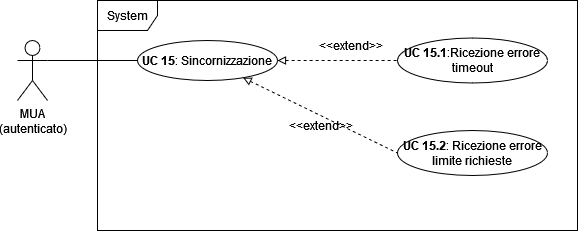
\includegraphics[width=0.85\textwidth]{sections/uc_imgs/UCS.png}
        \centering
        \caption{Diagramma UC S }
    \end{figure}
    \begin{itemize}
        \item \textbf{Attore principale}: MUA;
        \item \textbf{Descrizione}: il MUA richiede la sincronizzazione con gli oggetti del sistema;
        \item \textbf{Precondizioni}: l’account che il MUA gestisce è registrato nel sistema, e ha un connessione aperta con il sistema ed è autenticato;
        \item \textbf{Postcondizioni}: il MUA è sincronizzato con i dati presenti nel sistema;
        \item \textbf{Scenario principale}:
            \begin{enumerate}
                \item il MUA invia i dettagli necessari ad indentificare gli oggetti da Sincronizzare;
                \item il sistema invia al MUA gli aggiornamenti;
            \end{enumerate}
        \item \textbf{Inclusioni}: nessuna;
        \item \textbf{Generalizzazioni}: nessuna;
            % tho la sincronizzazione è fatta per oggetto con jmap
            %\begin{itemize}
            %    \item il MUA sincronizza contatti (\hyperref[sec:UC12]{UC 12});
            %    \item il MUA sincronizza eventi nel calendario (\hyperref[sec:UC13]{UC 13});
            %    \item il MUA sincronizza cartelle (\hyperref[sec:UC14]{UC 14});
            %\end{itemize}
        \item \textbf{Estensioni}: 
        \begin{itemize}
            \item il sistema ritorna un errore al MUA per timeout (\hyperref[sec:UC11.2]{UC 11.2}).
            \item il sistema ritorna un errore al MUA per limite richieste (\hyperref[sec:UC11.2]{UC 11.2}).

        \end{itemize}
    \end{itemize}


    \subsubsection{UC S.1 - Ricezione errore timeout} \label{sec:UCS.1}
    \begin{itemize}
        \item \textbf{Attore principale}: MUA;
        \item \textbf{Descrizione}: il sistema non riesce a sincronizzarsi perché il tempo necessario per completare l'operazione supera il limite di timeout;
        \item \textbf{Precondizioni}: il MUA sta usando la funzionalità sincronizzazione;
        \item \textbf{Postcondizioni}: il sistema non invia al MUA gli aggiornamenti, il MUA è stato notificato dell'errore;
        \item \textbf{Scenario principale}:
            \begin{enumerate}
                \item l'operazione richiesta supera il tempo massimo previsto dal sistema;
                \item il sistema non invia gli aggiornamenti e notifica il MUA dell'errore;
            \end{enumerate}
        \item \textbf{Inclusioni}: nessuna;
        \item \textbf{Generalizzazioni}: nessuna;
        \item \textbf{Estensioni}: nessuna.
    \end{itemize}

    \subsubsection{UC S.2 - Ricezione errore limite richieste} \label{sec:UCS.2}
    \begin{itemize}
        \item \textbf{Attore principale}: MUA;
        \item \textbf{Descrizione}: il sistema non riesce a sincronizzarsi perché il MUA supera la quantità massima di richieste al server;
        \item \textbf{Precondizioni}: il MUA sta usando la funzionalità sincronizzazione;
        \item \textbf{Postcondizioni}: il sistema non invia al MUA gli aggiornamenti, il MUA è stato notificato dell'errore;
        \item \textbf{Scenario principale}:
            \begin{enumerate}
                \item il MUA supera la quantità massima di richieste da mandare al sistema;
                \item il sistema non invia gli aggiornamenti e notifica il MUA dell'errore;
            \end{enumerate}
        \item \textbf{Inclusioni}: nessuna;
        \item \textbf{Generalizzazioni}: nessuna;
        \item \textbf{Estensioni}: nessuna.
    \end{itemize}



%     \subsubsection{UC 2.1 - Trasmettere richiesta di aggiornamento} \label{sec: UC 2.1}
%     \begin{itemize}
%         \item Attore: MUA;
%         \item Descrizione: il MUA deve poter richiedere un aggiornamento dei propri dati;
%         \item Scenario:
%         \begin{enumerate}
%         \item il MUA si connette con il server;
%         \item il MUA richiede nuovi dati.
%         \end{enumerate}
%         \item Estensioni: errore... %(\hyperref[sec: UC 1.4.1]{UC 1.4.1});
%         \item Precondizioni: il MUA si sta aggiornando con i nuovi dati;
%         \item Postcondizioni: il MUA ha ricevuto nuove informazioni.
%     \end{itemize}



%     \subsubsection{UC 3.1 - Creare una cartella} \label{sec: UC 3.1}
%     \begin{itemize}
%         \item Attore: MUA;
%         \item Descrizione: il MUA deve poter creare una cartella;
%         \item Scenario:
%             \begin{enumerate}
%             \item il MUA si connette con il server;
%             \item il MUA trasmette i dati necessari per creare la cartella; 
%             \item % scrivere trasmettere solo nome forse???
%             \end{enumerate}
%         \item Estensioni: Errore nome cartella
%         \item Precondizioni: il MUA sta creando una cartella;
%         \item Postcondizioni: è stata creata la cartella.
%     \end{itemize}

%     \subsubsection{UC 3.2 - Creare un contatto} \label{sec: UC 3.2}
%     \begin{itemize}
%         \item Attore: MUA;
%         \item Descrizione: il MUA deve poter creare un contatto;
%         \item Scenario:
%         \begin{enumerate}
%         \item il MUA si connette con il server;
%         \item il MUA trasmette i dati necessari per creare il contatto;
%         \end{enumerate}
%         \item Estensioni: errore...
%         \item Precondizioni: il MUA sta creando un contatto;
%         \item Postcondizioni: è stata creata il contatto.
%     \end{itemize}

%     \subsubsection{UC 3.3 - Creare una condivisione} \label{sec: UC 3.3}
%     \begin{itemize}
%         \item Attore: MUA;
%         \item Descrizione: il MUA deve poter creare una condivisione di una cartella;
%         \item Scenario:
%         \begin{enumerate}
%         \item il MUA si connette con il server;
%         \item il MUA trasmette i dati necessari per creare la condivisione della cartella.
%         \end{enumerate}
%         \item Estensioni: errore...
%         \item Precondizioni: l’account che il MUA gestisce è registrato nel sistema ed è autenticato;
%         \item Postcondizioni: è stata creata la condivisione di una cartella.
%     \end{itemize}

%     \subsubsection{UC 3.4 - Creare un evento} \label{sec: UC 3.4}
%     \begin{itemize}
%         \item Attore: MUA;
%         \item Descrizione: il MUA deve poter creare un evento;
%         \item Scenario:
%         \begin{enumerate}
%         \item il MUA si connette con il server;
%         \item il MUA trasmette i dati necessari per creare un evento.
%         \end{enumerate}
%         \item Estensioni: errore...
%         \item Precondizioni: il MUA sta creando un evento;
%         \item Postcondizioni: è stato creato l'evento.
%     \end{itemize}

%     \subsection{UC 4 - Modificare un oggetto} \label{sec: UC 4}
%     \begin{itemize}
%         \item Attore: MUA;
%         \item Descrizione: il MUA deve poter modificare un oggetto specifico;
%         \item Scenario principale:
%             \begin{enumerate}
%                 \item 
%             \end{enumerate}
%         \item Generalizzazioni:
%             \begin{itemize}
%             \item il MUA modifica una cartella (\hyperref[sec: UC 4.1]{UC 4.1});
%             \item il MUA modifica un contatto (\hyperref[sec: UC 4.2]{UC 4.2});
%             \item il MUA mofidica una condivisione (\hyperref[sec: UC 4.3]{UC 4.3});
%             \item il MUA modifica un evento (\hyperref[sec: UC 4.4]{UC 4.4}).
%             \end{itemize}
%         \item Estensioni: errore...
%         \item Precondizioni: l’account che il MUA gestisce è registrato nel sistema ed è autenticato;
%         \item Postcondizioni: è stato modificato l’oggetto desiderato.
%     \end{itemize}

%     \subsubsection{UC 4.1 - Modificare una cartella} \label{sec: UC 4.1}
%     \begin{itemize}
%         \item Attore: MUA;
%         \item Descrizione: il MUA deve poter modificare una cartella;
%         \item Scenario:
%         \begin{enumerate}
%         \item il MUA si connette con il server;
%         \item Il MUA trasmette i dati necessari per modificare la cartella.
%         \end{enumerate}
%         \item Estensioni: errore...
%         \item Precondizioni: il MUA sta modificando una cartella;
%         \item Postcondizioni: è stata modificata la cartella.
%     \end{itemize}

%     \subsubsection{UC 4.2 - Modificare un contatto} \label{sec: UC 4.2}
%     \begin{itemize}
%         \item Attore: MUA;
%         \item Descrizione: il MUA deve poter modificare un contatto;
%         \item Scenario:
%         \begin{enumerate}
%         \item il MUA si connette con il server;
%         \item Il MUA trasmette i dati necessari per modificare il contatto.
%         \end{enumerate}
%         \item Estensioni: errore...
%         \item Precondizioni: il MUA sta modificando un contatto;
%         \item Postcondizioni: è stato modificato il contatto.
%     \end{itemize}

%     \subsubsection{UC 4.3 - Modificare una condivisione} \label{sec: UC 4.3}
%     \begin{itemize}
%         \item Attore: MUA;
%         \item Descrizione: il MUA deve poter modificare una condivisione di una cartella;
%         \item Scenario:
%         \begin{enumerate}
%         \item il MUA si connette con il server;
%         \item Il MUA trasmette i dati necessari per modificare la condivisione di una cartella.
%         \end{enumerate}
%         \item Estensioni: errore...
%         \item Precondizioni: il MUA sta modificando una condivisione di una cartella;
%         \item Postcondizioni: è stata modificata la condivisione di una cartella.
%     \end{itemize}

%     \subsubsection{UC 4.4 - Modificare un evento} \label{sec: UC 4.4}
%     \begin{itemize}
%         \item Attore: MUA;
%         \item Descrizione: il MUA deve poter modificare un evento;
%         \item Scenario:
%         \begin{enumerate}
%         \item il MUA si connette con il server;
%         \item Il MUA trasmette i dati necessari per modificare un evento.
%         \end{enumerate}
%         \item Estensioni: 
%         \begin{itemize}
%             \item Errore dimensioni evento;
%         \end{itemize}
%         \item Precondizioni: il MUA sta modificando un evento;
%         \item Postcondizioni: è stato modificato l'evento.
%     \end{itemize}

%  

%     %creazione cartella problema nome
%     \paragraph{UC Errore nome cartella} \label{sec: UC 11.4.2.1}
%     \begin{itemize}
%         \item Attore: MUA;
%         \item Descrizione: il MUA deve ricevere un messaggio di errore adeguato quando si tenta la creazione di una cartella con lo stesso nome e la stessa cartella padre di un'altra;
%         \item Scenario:
%         \begin{enumerate}
%         \item il MUA riceve il messaggio di errore;
%         \end{enumerate}   
%         \item Precondizioni: 
%         \begin{enumerate}
%             \item il MUA ha trasmesso il nome per la creazione della cartella;
%             \item esiste già una cartella con lo stesso nome e la stessa cartella padre;
%         \end{enumerate}
%         \item Postcondizioni: il MUA ha ricevuto un messaggio di errore.
%     \end{itemize}

%     %modificare una cartella (tho anche per creare c'è)
%     \paragraph{UC Errore dimensioni cartella} \label{sec: UC 11.4.2.1}
%     \begin{itemize}
%         \item Attore: MUA;
%         \item Descrizione: il MUA deve ricevere un messaggio di errore adeguato quando la modifica di una o più caratteristiche di una cartella superano i limiti di dimensione stabiliti;
%         \item Scenario:
%         \begin{enumerate}
%         \item il MUA riceve il messaggio di errore;
%         \end{enumerate}   
%         \item Precondizioni: 
%         \begin{enumerate}
%             \item il MUA ha trasmesso i dati per la modifica di una cartella;
%             \item una o più caratteristiche di una cartella superano i limiti di dimensione stabiliti;
%         \end{enumerate}
%         \item Postcondizioni: il MUA ha ricevuto un messaggio di errore.
%     \end{itemize}

%     %modificare una cartella (tho anche per creare c'è)
%     \paragraph{UC Errore validità cartella} \label{sec: UC 11.4.2.1}
%     \begin{itemize}
%         \item Attore: MUA;
%         \item Descrizione: il MUA deve ricevere un messaggio di errore adeguato quando la modifica di una o più caratteristiche di una cartella riporta un formato non valido;
%         \item Scenario:
%         \begin{enumerate}
%         \item il MUA riceve il messaggio di errore;
%         \end{enumerate}   
%         \item Precondizioni: 
%         \begin{enumerate}
%             \item il MUA ha trasmesso i dati per la modifica di una cartella;
%             \item una o più caratteristiche di una cartella  non sono valide;
%         \end{enumerate}
%         \item Postcondizioni: il MUA ha ricevuto un messaggio di errore.
%     \end{itemize}


%     %modificare una cartella (tho anche per eliminare c'è)
%     %troppo? sarebbe una ricerca per id
%     \paragraph{UC Errore esistenza cartella} \label{sec: UC 11.4.2.1}
%     \begin{itemize}
%         \item Attore: MUA;
%         \item Descrizione: il MUA deve ricevere un messaggio di errore adeguato quando la ricerca della cartella che si intende modificare fallisce;
%         \item Scenario:
%         \begin{enumerate}
%         \item il MUA riceve il messaggio di errore;
%         \end{enumerate}   
%         \item Precondizioni: 
%         \begin{enumerate}
%             \item il MUA ha trasmesso i dati per la modifica di una cartella;
%             \item non viene trovata la cartella;
%         \end{enumerate}
%         \item Postcondizioni: il MUA ha ricevuto un messaggio di errore.
%     \end{itemize}

%     %eliminazione cartella con email
%     \paragraph{UC Errore cartella contenente email} \label{sec: UC 11.4.2.1}
%     \begin{itemize}
%         \item Attore: MUA;
%         \item Descrizione: il MUA deve ricevere un messaggio di errore adeguato quando l'eliminazione di una cartella non è andata a buon fine a causa di una o più email presenti all'interno di quella cartella;
%         \item Scenario:
%         \begin{enumerate}
%         \item il MUA riceve il messaggio di errore;
%         \end{enumerate}   
%         \item Precondizioni: 
%         \begin{enumerate}
%             \item il MUA ha trasmesso i dati per l'emilinazione di una cartella ;
%             \item la cartella contiene una o più email;
%         \end{enumerate}
%         \item Postcondizioni: il MUA ha ricevuto un messaggio di errore.
%     \end{itemize}

%     %eliminazione cartella con cartelle
%     \paragraph{UC Errore cartella contenente cartelle} \label{sec: UC 11.4.2.1}
%     \begin{itemize}
%         \item Attore: MUA;
%         \item Descrizione: il MUA deve ricevere un messaggio di errore adeguato quando l'eliminazione di una cartella non è andata a buon fine a causa di una o più cartelle presenti all'interno di quella cartella;
%         \item Scenario:
%         \begin{enumerate}
%         \item il MUA riceve il messaggio di errore;
%         \end{enumerate}   
%         \item Precondizioni: 
%         \begin{enumerate}
%             \item il MUA ha trasmesso i dati per l'emilinazione di una cartella ;
%             \item la cartella contiene una o più cartelle;
%         \end{enumerate}
%         \item Postcondizioni: il MUA ha ricevuto un messaggio di errore.
%     \end{itemize}

%     %modificare un evento/ creazione
%     \paragraph{UC Errore dimensioni evento} \label{sec: UC 11.4.2.1}
%     \begin{itemize}
%         \item Attore: MUA;
%         \item Descrizione: il MUA deve ricevere un messaggio di errore adeguato quando la modifica di una o più caratteristiche di un evento superano i limiti di dimensione stabiliti;
%         \item Scenario:
%         \begin{enumerate}
%         \item il MUA riceve il messaggio di errore;
%         \end{enumerate}   
%         \item Precondizioni: 
%         \begin{enumerate}
%             \item il MUA ha trasmesso i dati per la modifica di un evento;
%             \item una o più caratteristiche di un evento superano i limiti di dimensione stabiliti;
%         \end{enumerate}
%         \item Postcondizioni: il MUA ha ricevuto un messaggio di errore.
%     \end{itemize}

%     %modificare un contatto / creazione
%     \paragraph{UC Errore dimensioni contatto} \label{sec: UC 11.4.2.1}
%     \begin{itemize}
%         \item Attore: MUA;
%         \item Descrizione: il MUA deve ricevere un messaggio di errore adeguato quando la modifica di una o più caratteristiche di un contatto superano i limiti di dimensione stabiliti;
%         \item Scenario:
%         \begin{enumerate}
%         \item il MUA riceve il messaggio di errore;
%         \end{enumerate}   
%         \item Precondizioni: 
%         \begin{enumerate}
%             \item il MUA ha trasmesso i dati per la modifica di un contatto;
%             \item una o più caratteristiche di un contatto superano i limiti di dimensione stabiliti;
%         \end{enumerate}
%         \item Postcondizioni: il MUA ha ricevuto un messaggio di errore.
%     \end{itemize}




%             %%%% COSE UTILI %%%%
%     \paragraph{UC  errore} \label{sec: UC 11.4.2.1}
%     \begin{itemize}
%         \item Attore: MUA;
%         \item Descrizione: il MUA deve ricevere un messaggio di errore adeguato quando l'eliminazione degli elementi non è andata a buon fine;
%         \item Scenario:
%         \begin{enumerate}
%         \item il MUA riceve il messaggio di errore
%         \end{enumerate}   
%         \item Precondizioni: il MUA ha trasmesso ...;
%         \item Postcondizioni: il MUA ha ricevuto un messaggio d'errore.
%     \end{itemize}

%     \subsection{UC 18 - Stress test}
% \begin{itemize}
%     \item Attore: developer Zextras;
%     \item Descrizione: l'utente deve poter fare degli stess test per misurare le performance del prodotto;
%     \item Scenario principale:
%         \begin{enumerate}
%         \item l'utente avvia uno o una serie di stress test. 
%         \end{enumerate}
%     \item Precondizioni: l'utente vuole avviare degli stess test;
%     \item Postcondizioni: l'utente visualizza i risultati dei test.
% \end{itemize}

   

    
